\subsubsection{Logistic map (LOG)} \label{subsubsec:log}

Logistic map is representative of the very large family of quadratic maps. 
\begin{equation}\label{eq:logimap}
 x_{n+1}~=~4~x_n~(1-x_n) \ ,
\end{equation}
with $x_n\in\mathcal{R}$.
 
Figs. \ref{fig:LOGdecimal} (a) to (f) show the statistical properties of LOG map in floating point and decimal numbers representation. This map does not show the anomalies pointed above for the tent map. For $P\geq 10$ the values of $H_{hist}$, $H_{BP}$ and $C_{BP}$ remains almost identical to the values for the floating point representation. Their values are: $<H_{hist}>=0.8621$ with variance $\sigma_{H_{hist}}=0.062 \times 10^{-6}$; $<H_{BP}>=0.6292$ with variance $\sigma_{H_{BP}}=0.060 \times 10^{-6}$; $<C_{BP}>=0.4842$ with variance $\sigma_{C_{BP}}=0.0195 \times 10^{-6}$. Missing patterns stabilize in $645$ for $P \geq 8$ making $H_{BP}$ to rise to its floating point value $<H_{BP}>=0.629$ with variance $\sigma_{H_{BP}}=0.060 \times 10^{-8}$. Note again that the stable value of mission patters missing patterns $645$ makes the optimum $H_{BP} \leq ln(75)/ln(720) \simeq 0.65$. Then $P=10$ is the most convenient choice because an increase in the number of decimal figures does not improve the statistical properties. 
Figs. \ref{fig:LOGbin} show the corresponding figures for binary representations. The histogram entropy $H_{hist}$ does not reach its floating point value within the maximum number of bits used. In the case of missing patterns the stable number $645$ is obtained with $B \geq 25$. It means that using $B=25$ one obtains a time series with good statistical properties regarding the missing patterns, but distribution among the allowed binary values is not as uniform as can be obtained with a higher value of $B$. 

\begin{figure}
	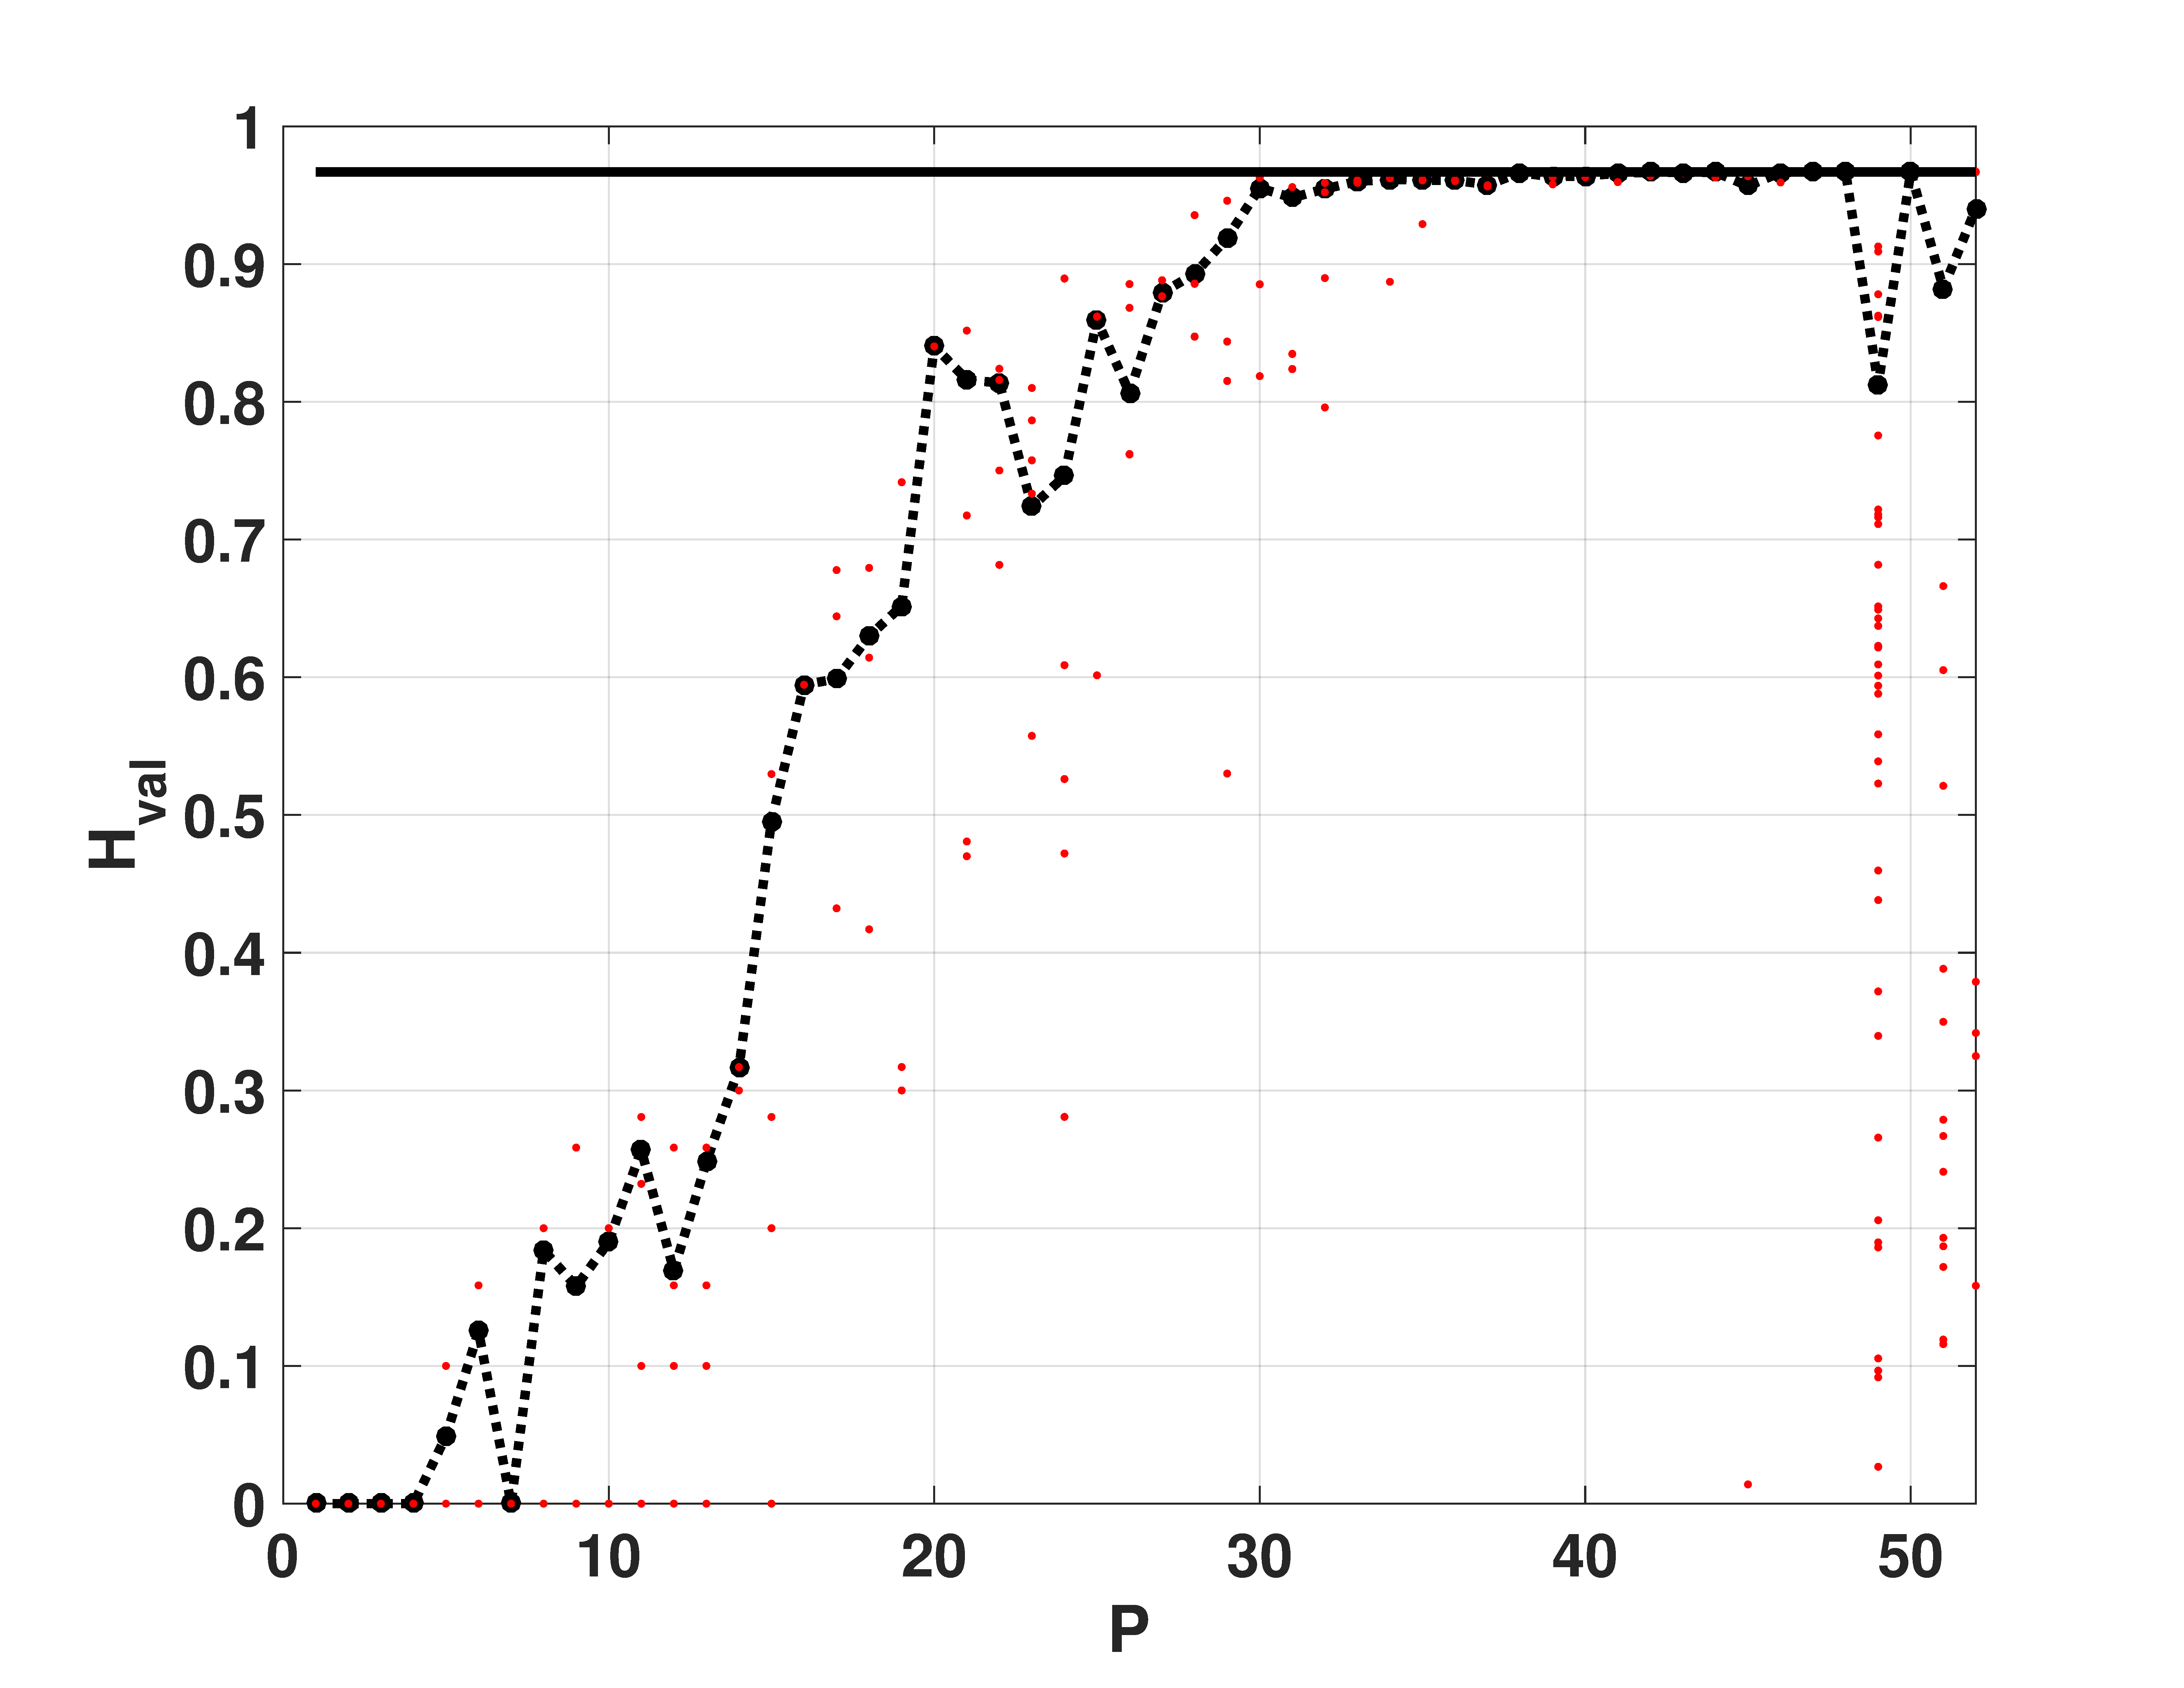
\includegraphics[width=.32\textwidth]{Hval_Logistico}
	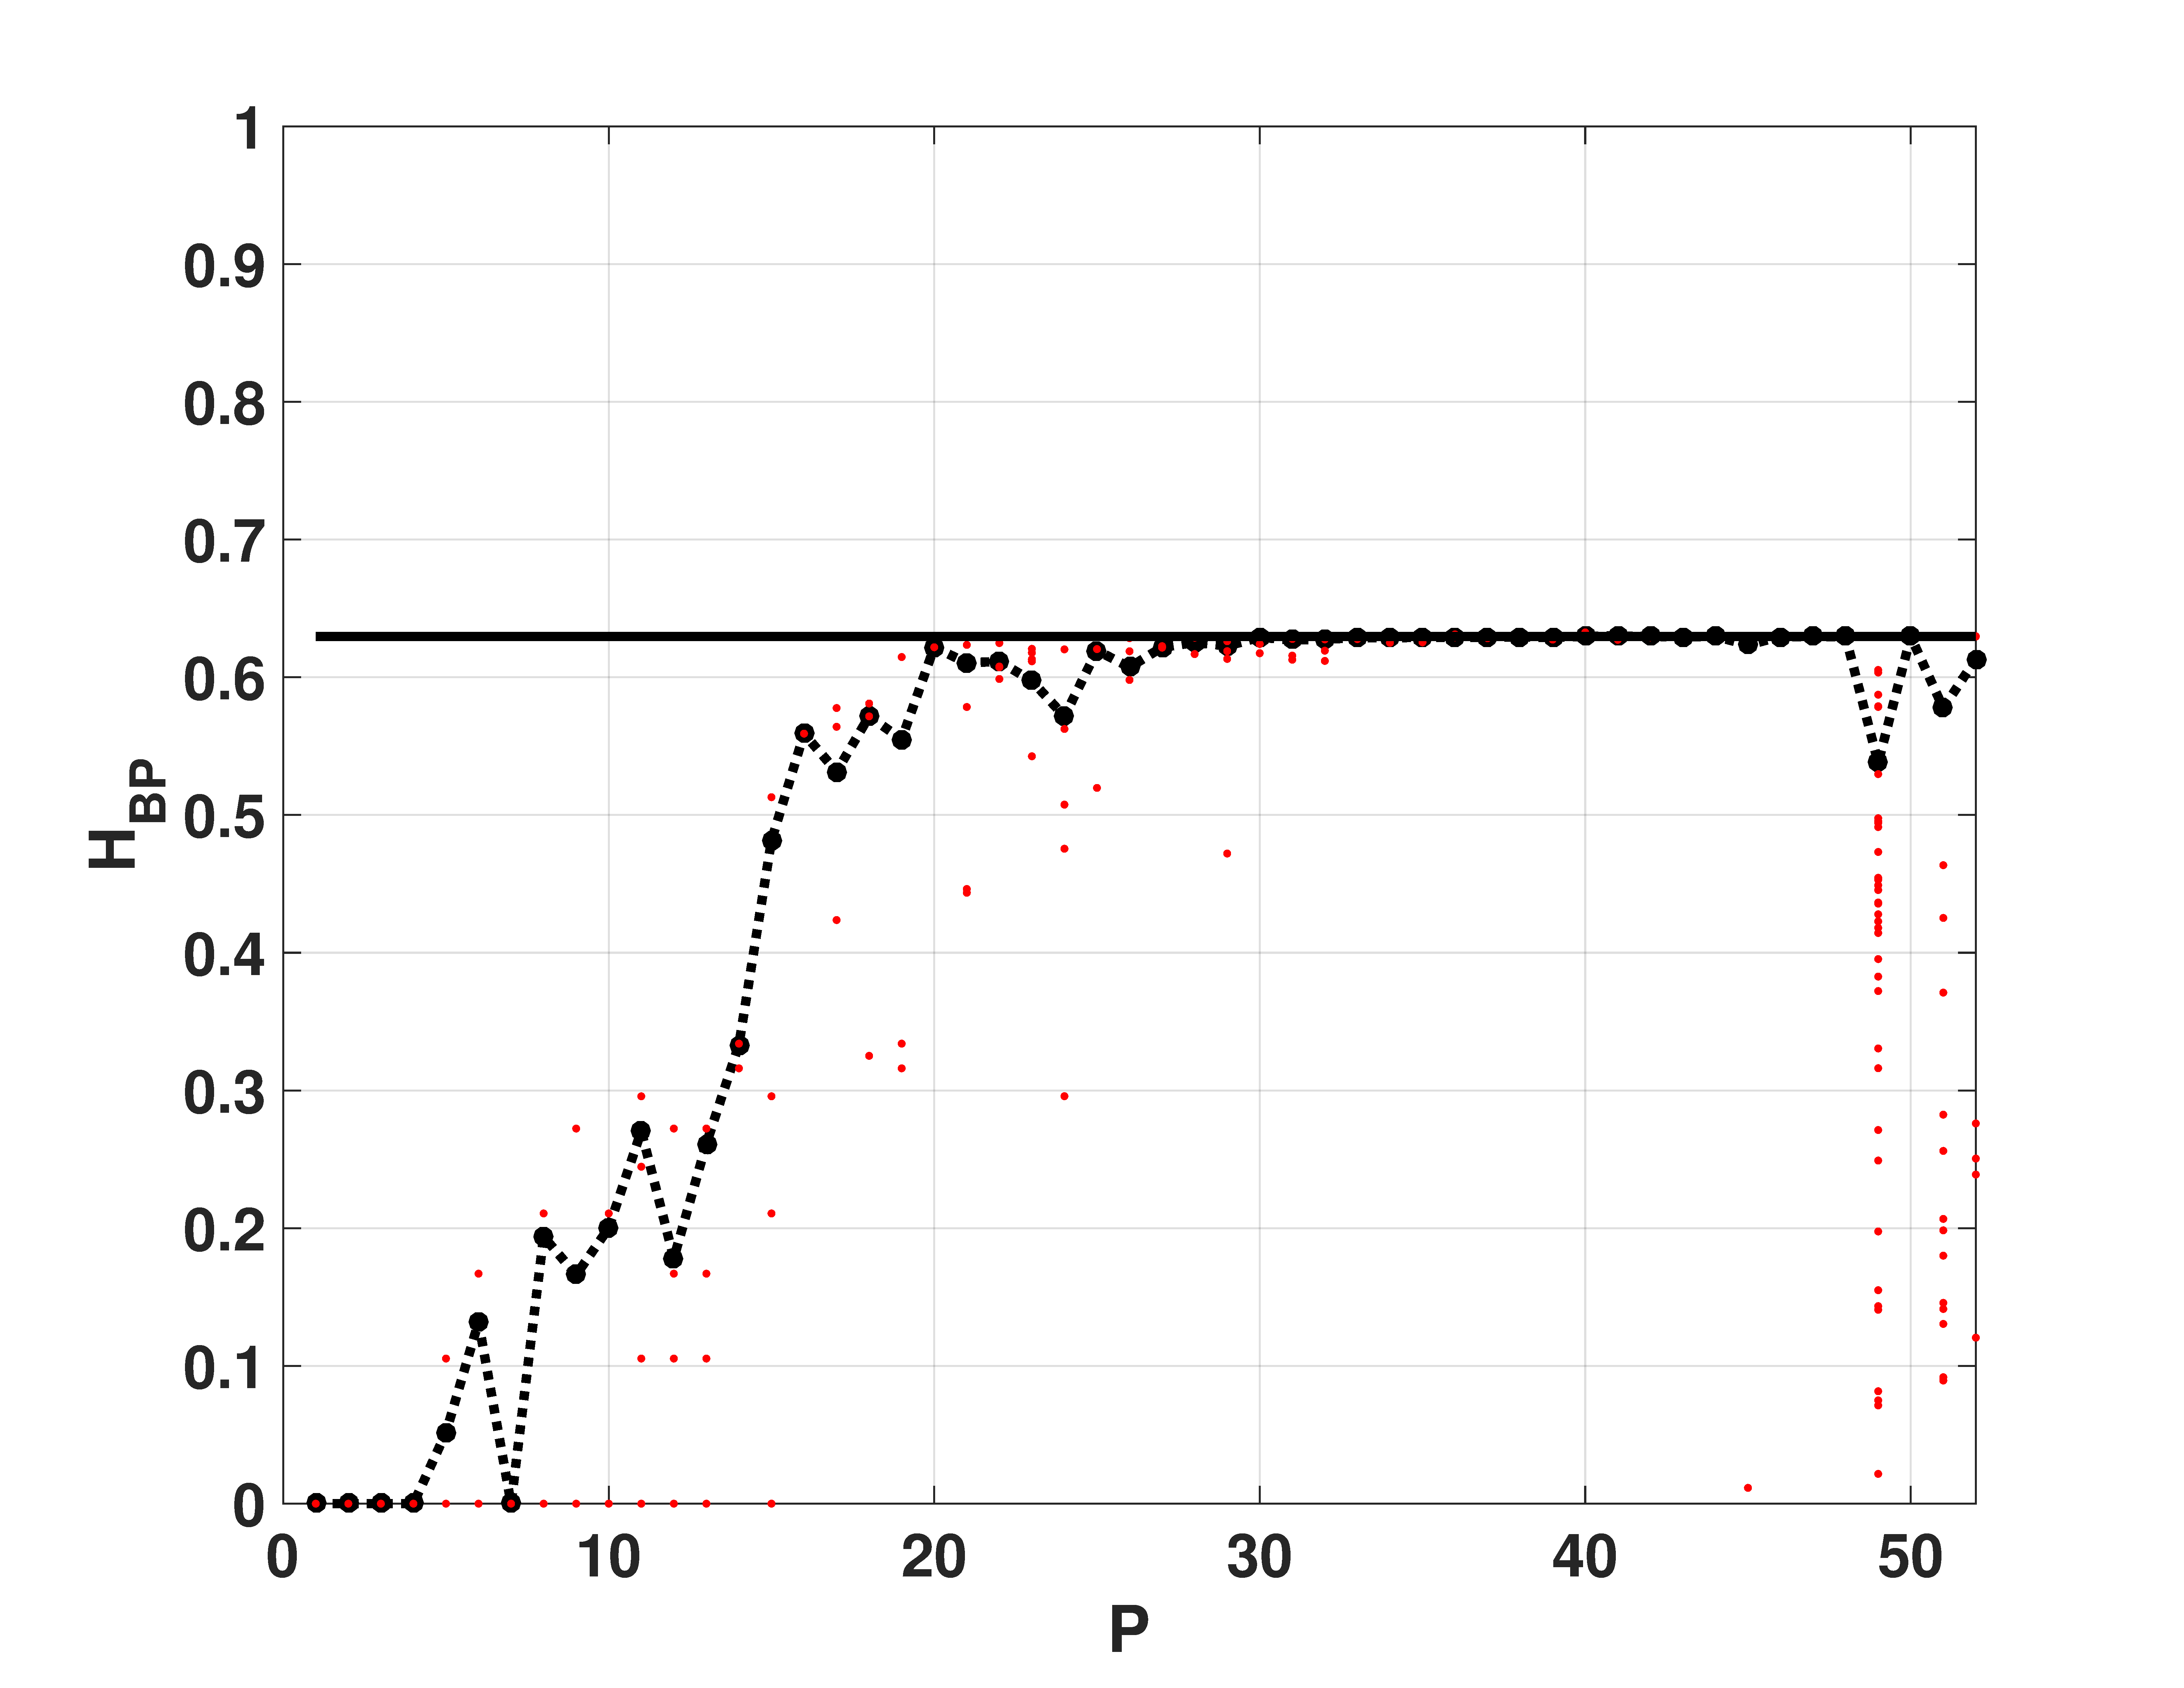
\includegraphics[width=.32\textwidth]{Hbp_Logistico}
	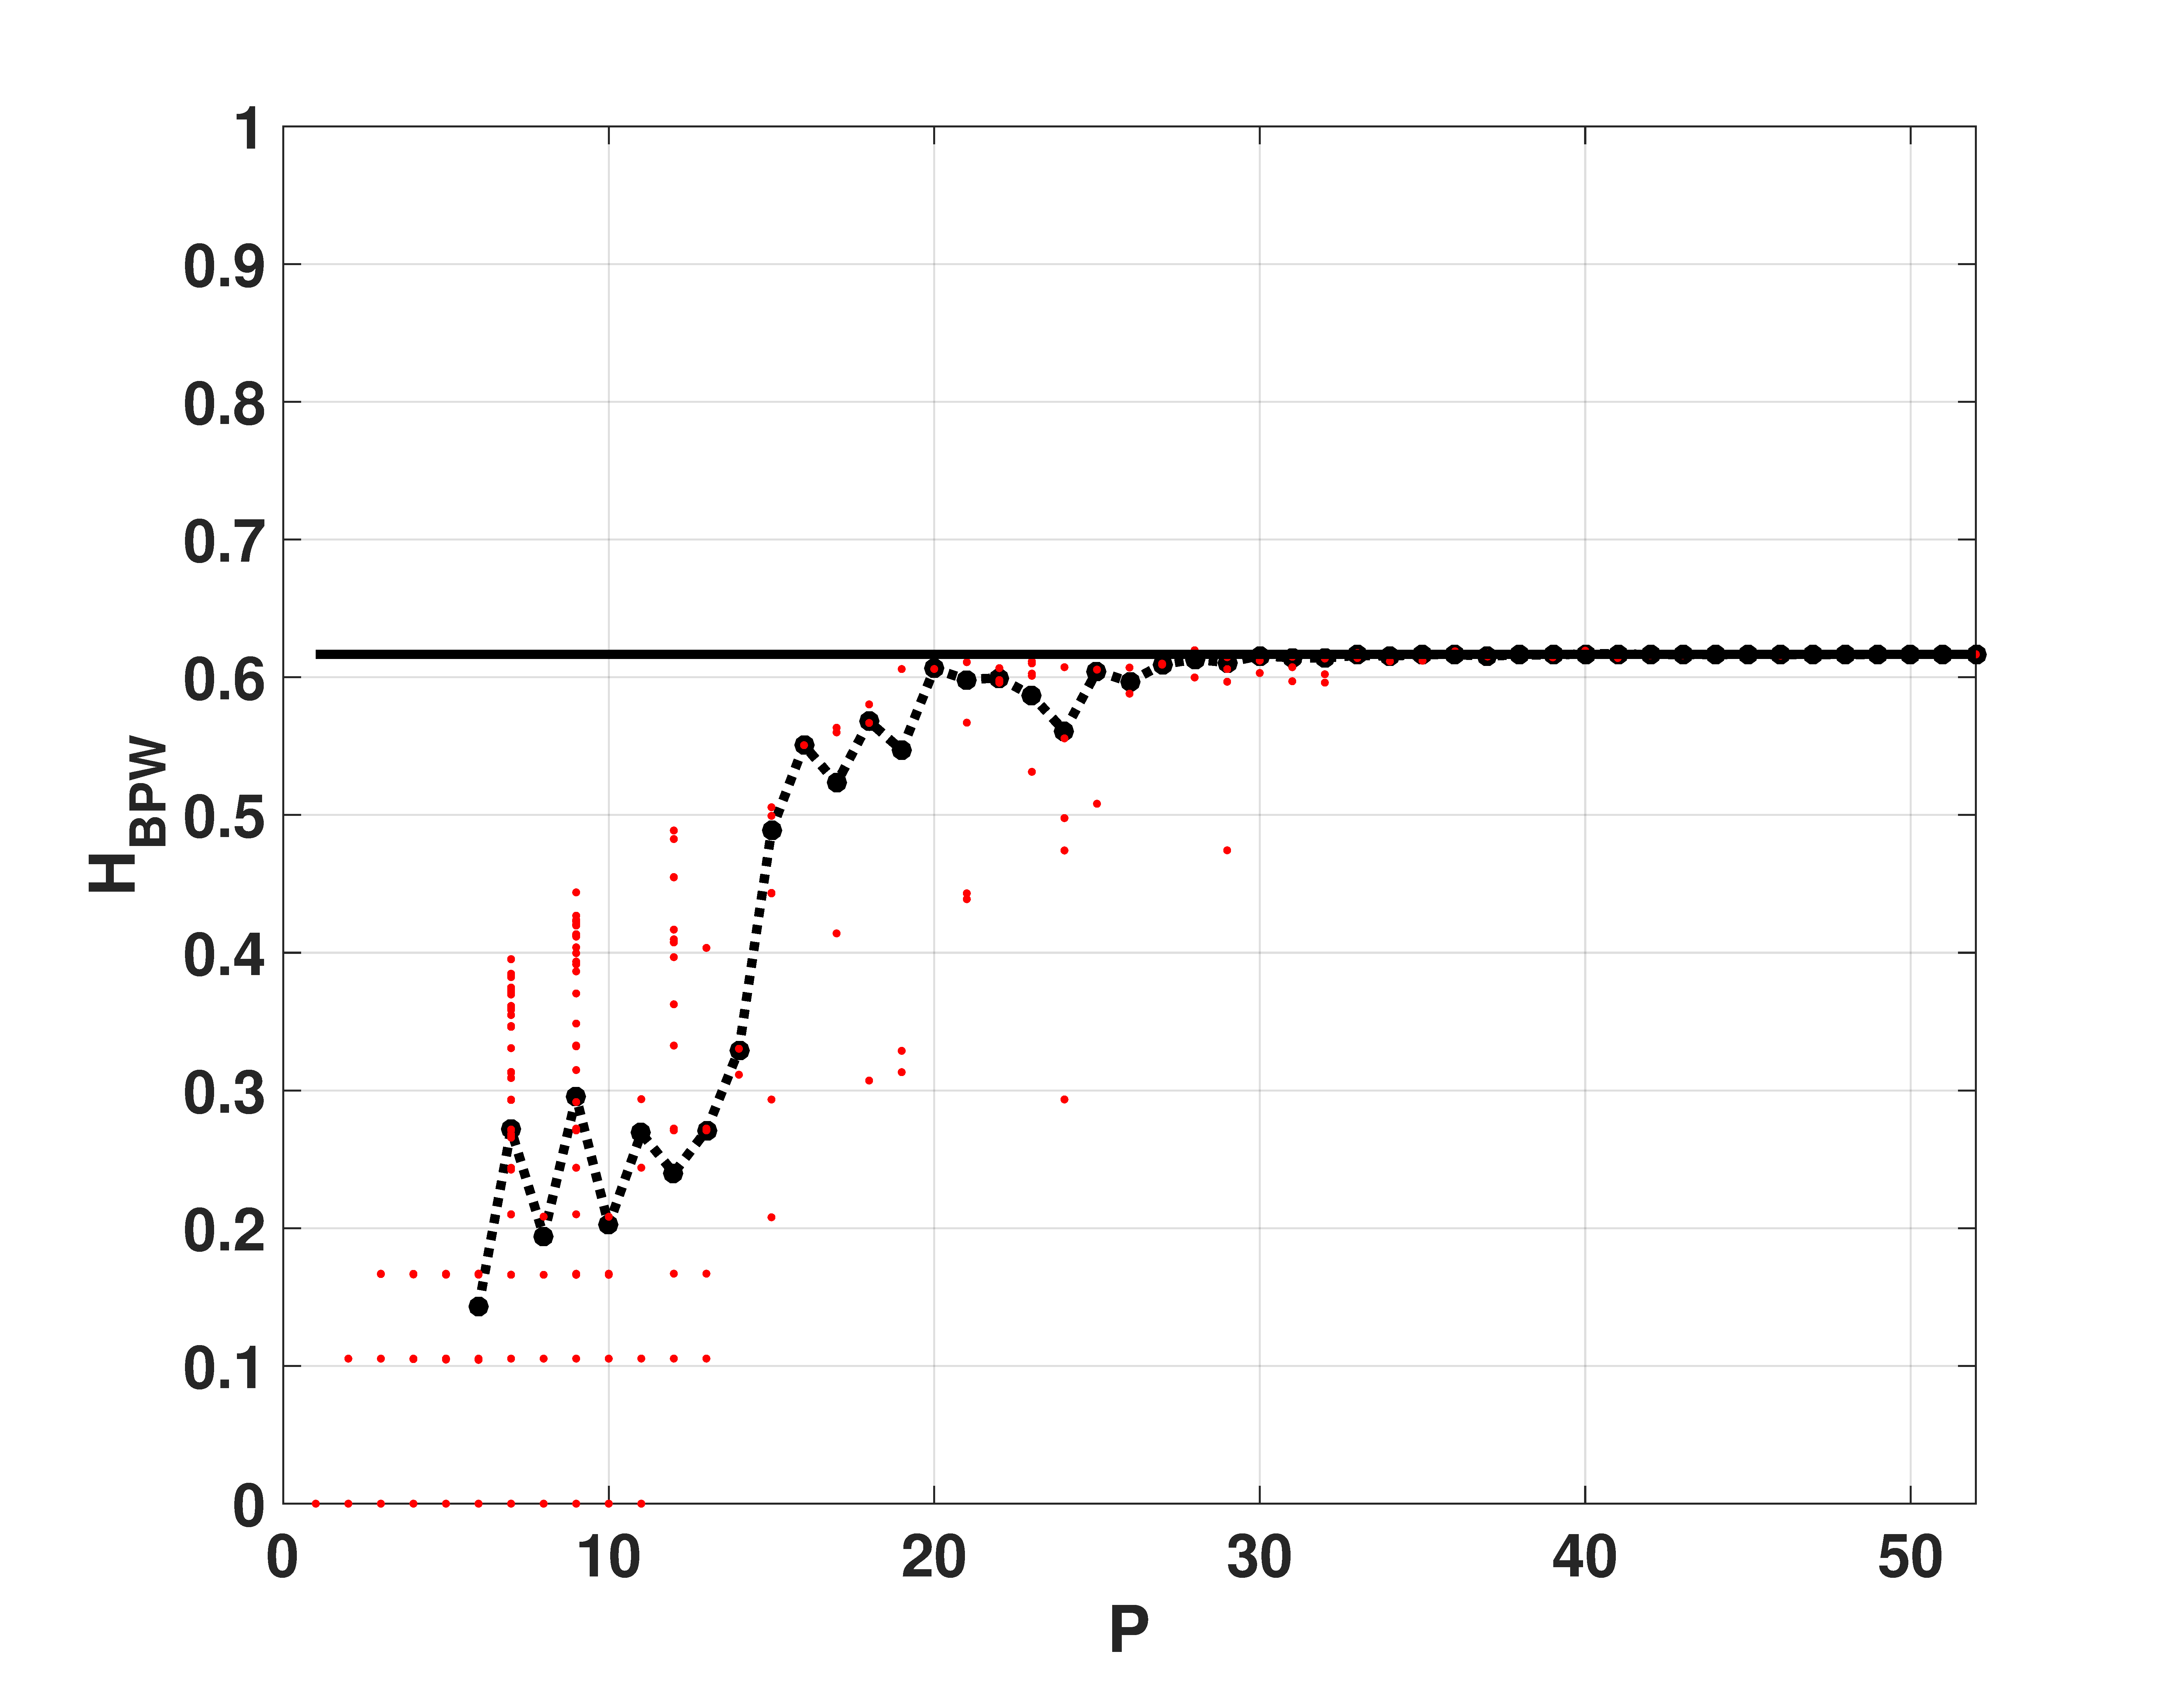
\includegraphics[width=.32\textwidth]{Hbpw_Logistico}
	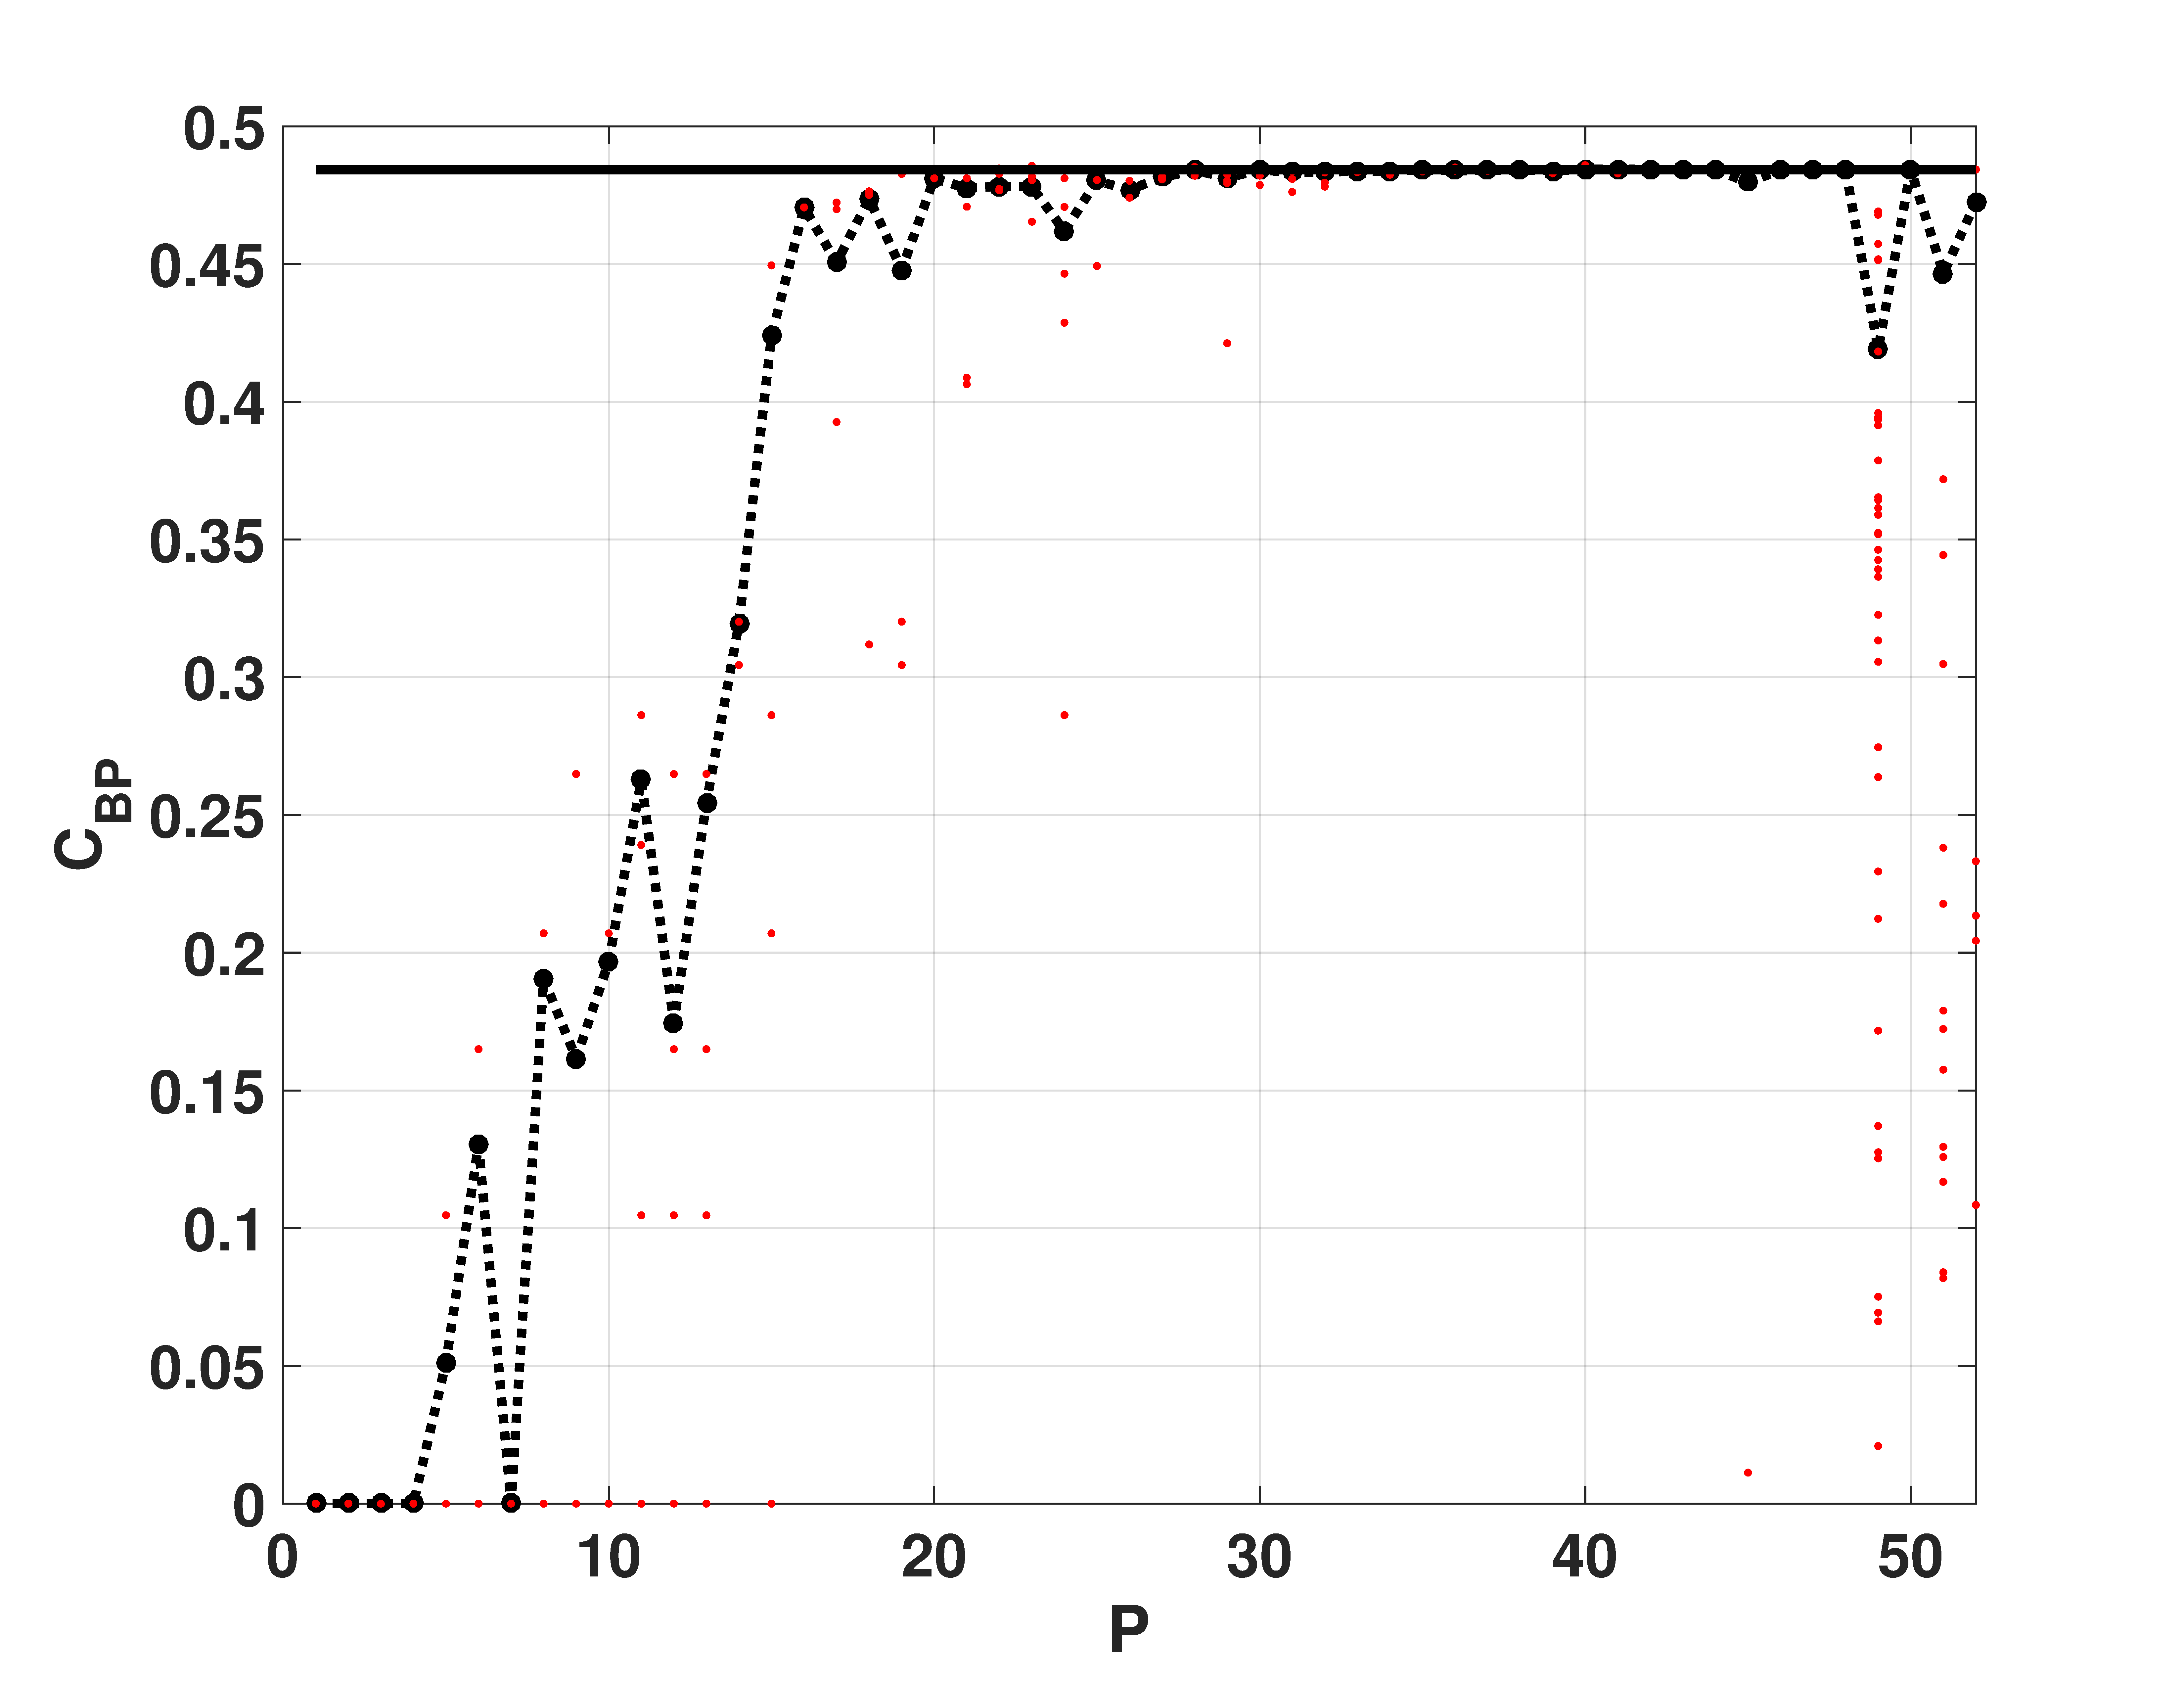
\includegraphics[width=.32\textwidth]{Cbp_Logistico}
	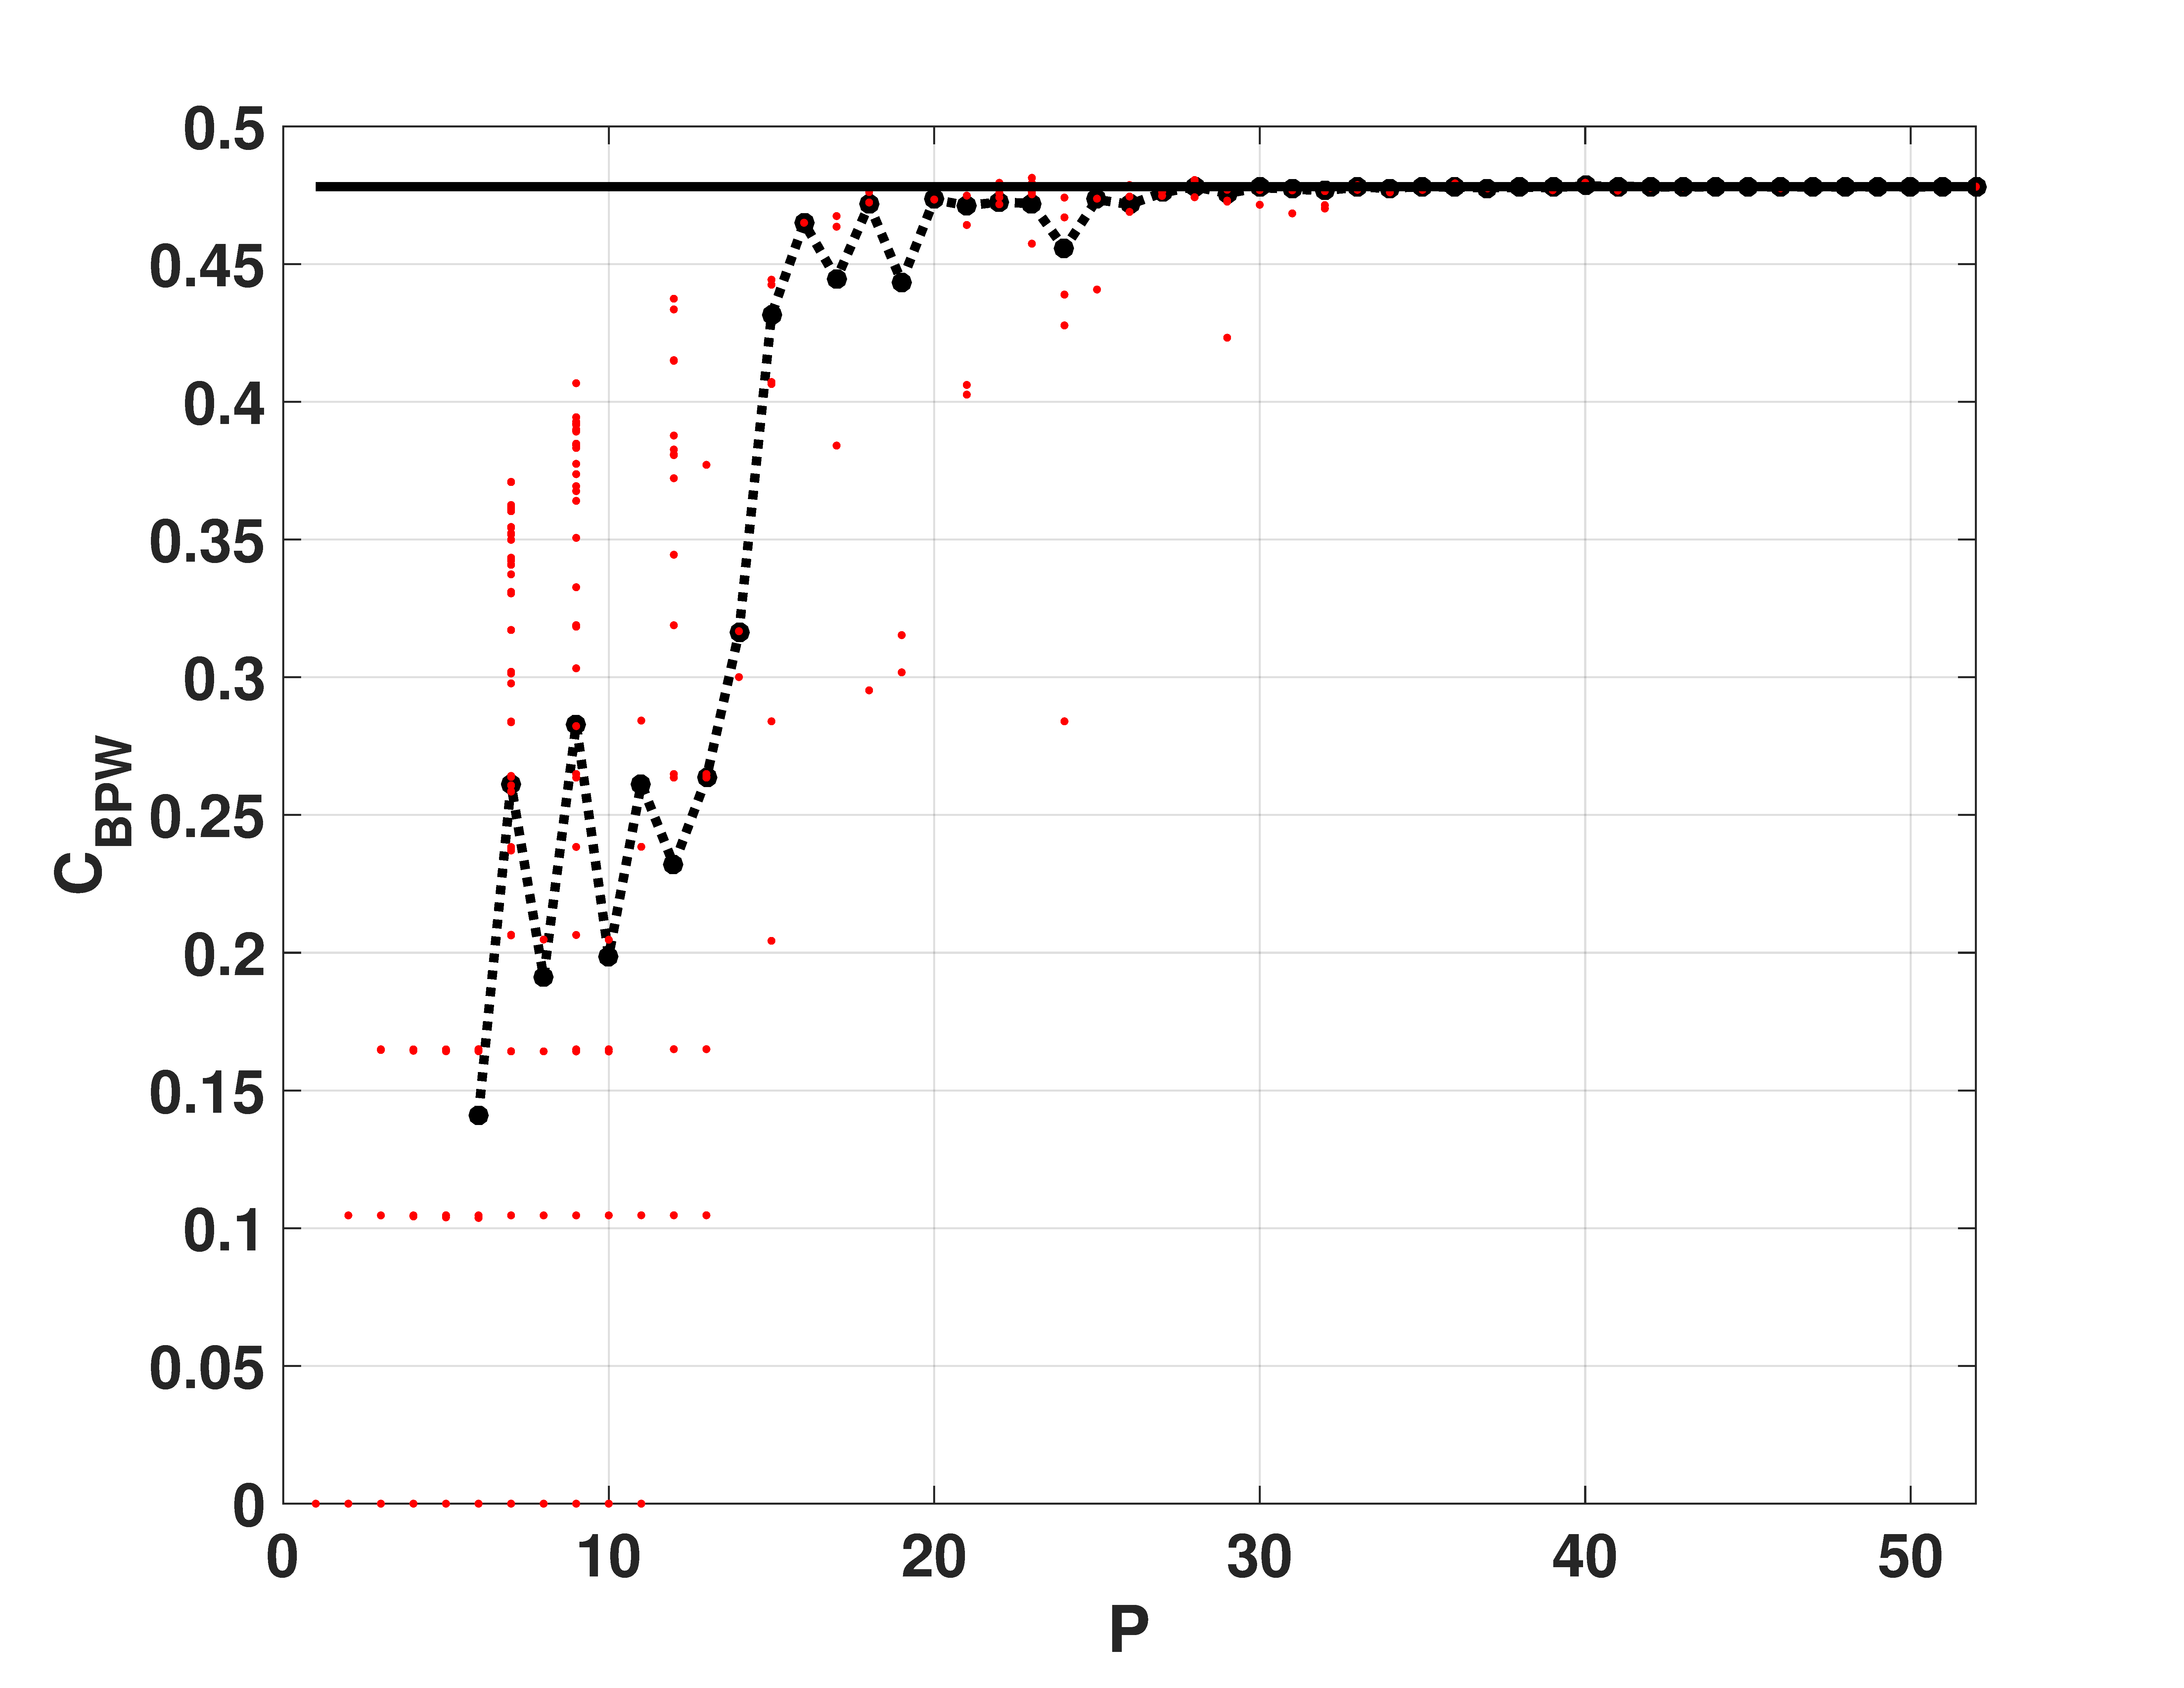
\includegraphics[width=.32\textwidth]{Cbpw_Logistico}
	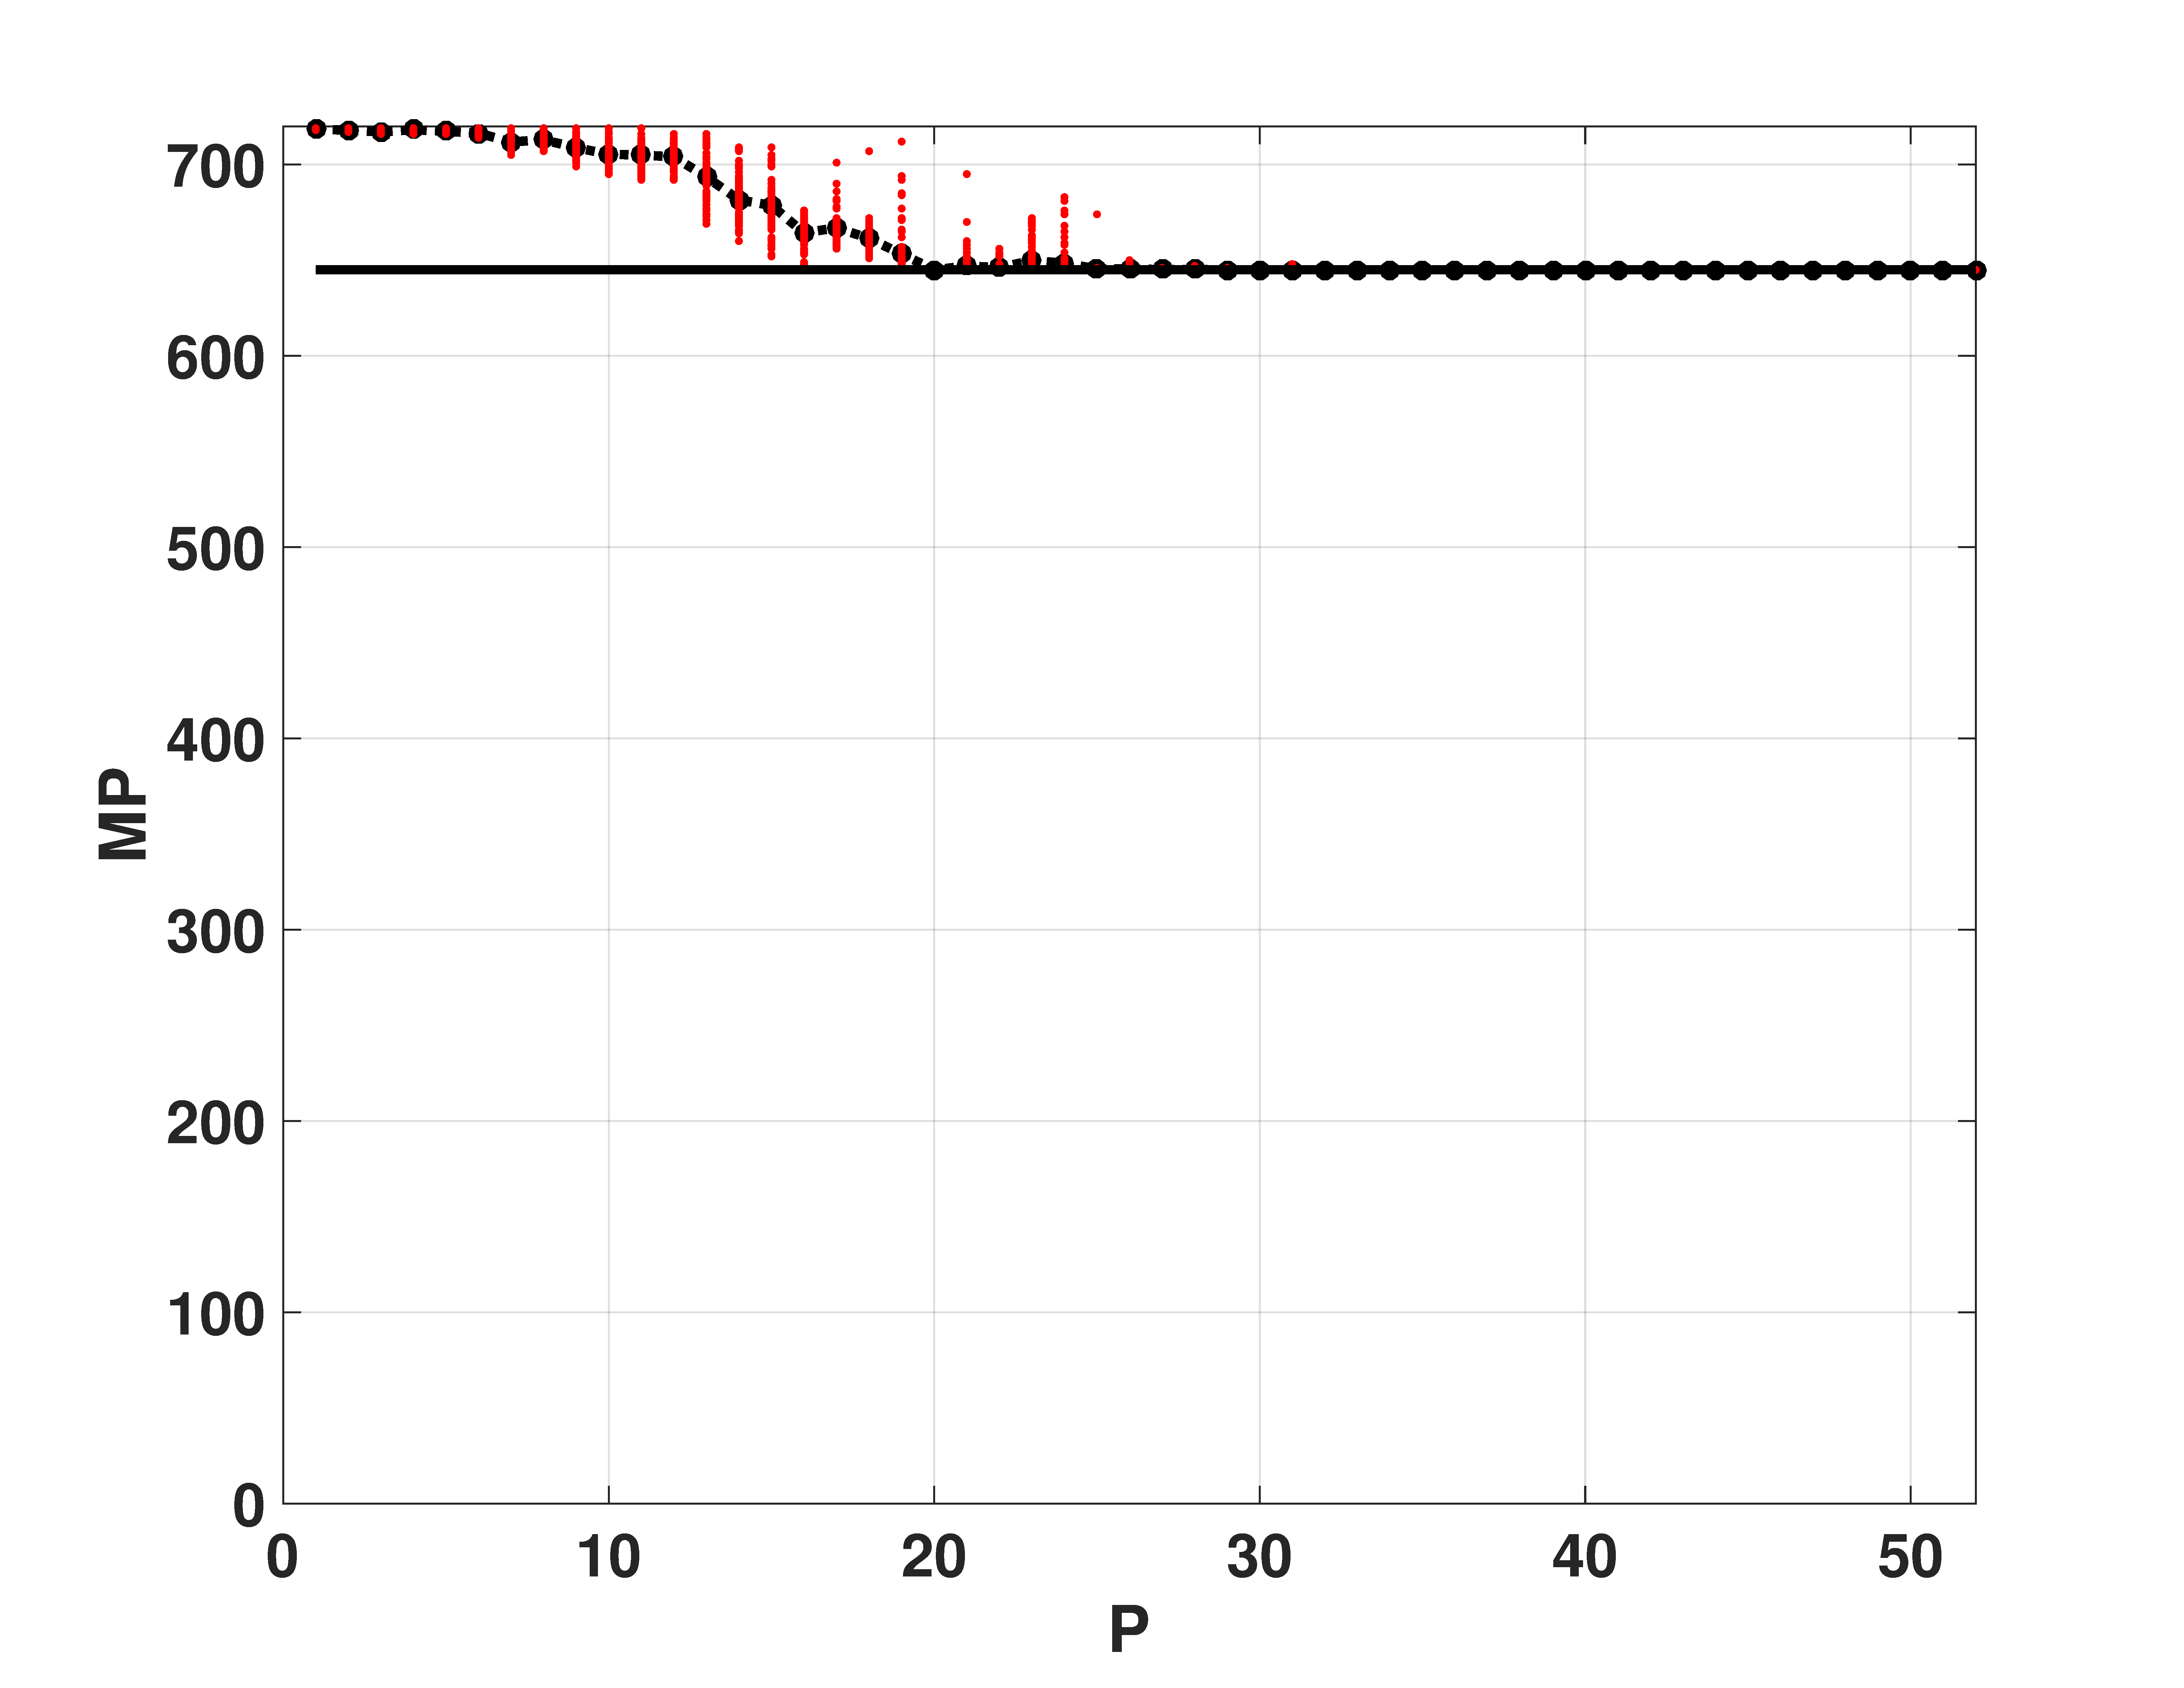
\includegraphics[width=.32\textwidth]{MP_Logistico}
	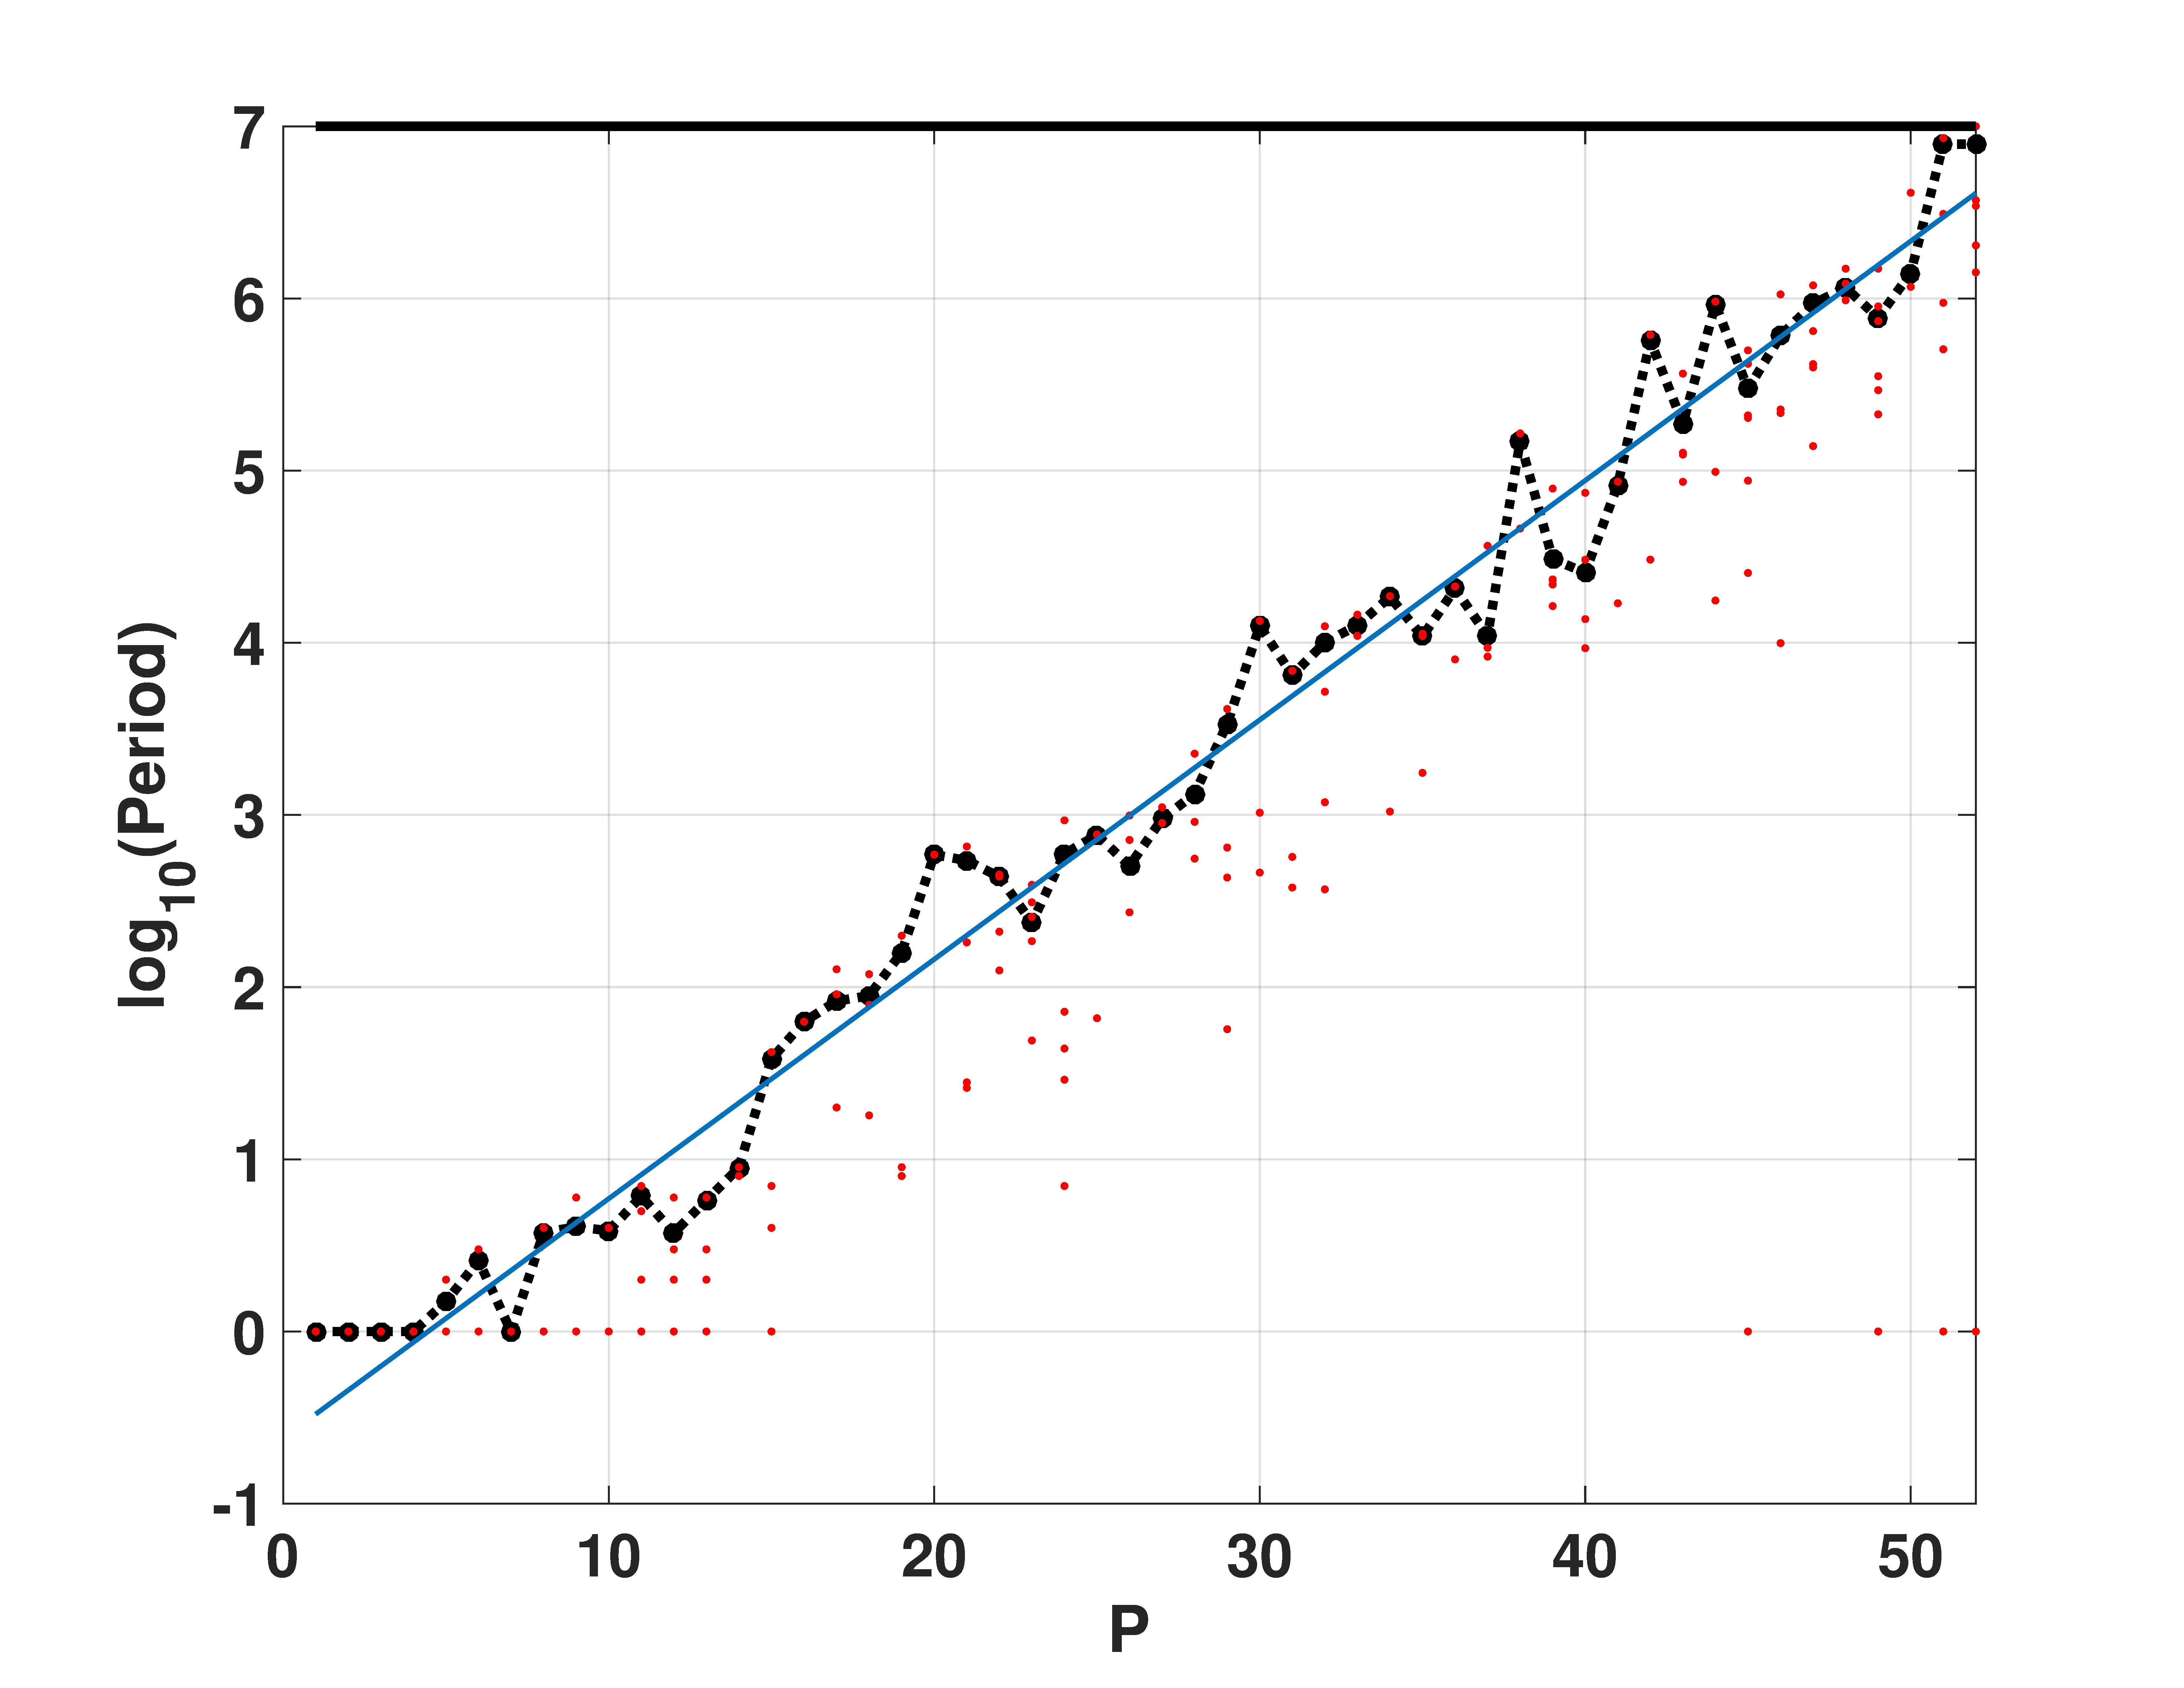
\includegraphics[width=.32\textwidth]{Period_Logistico}
	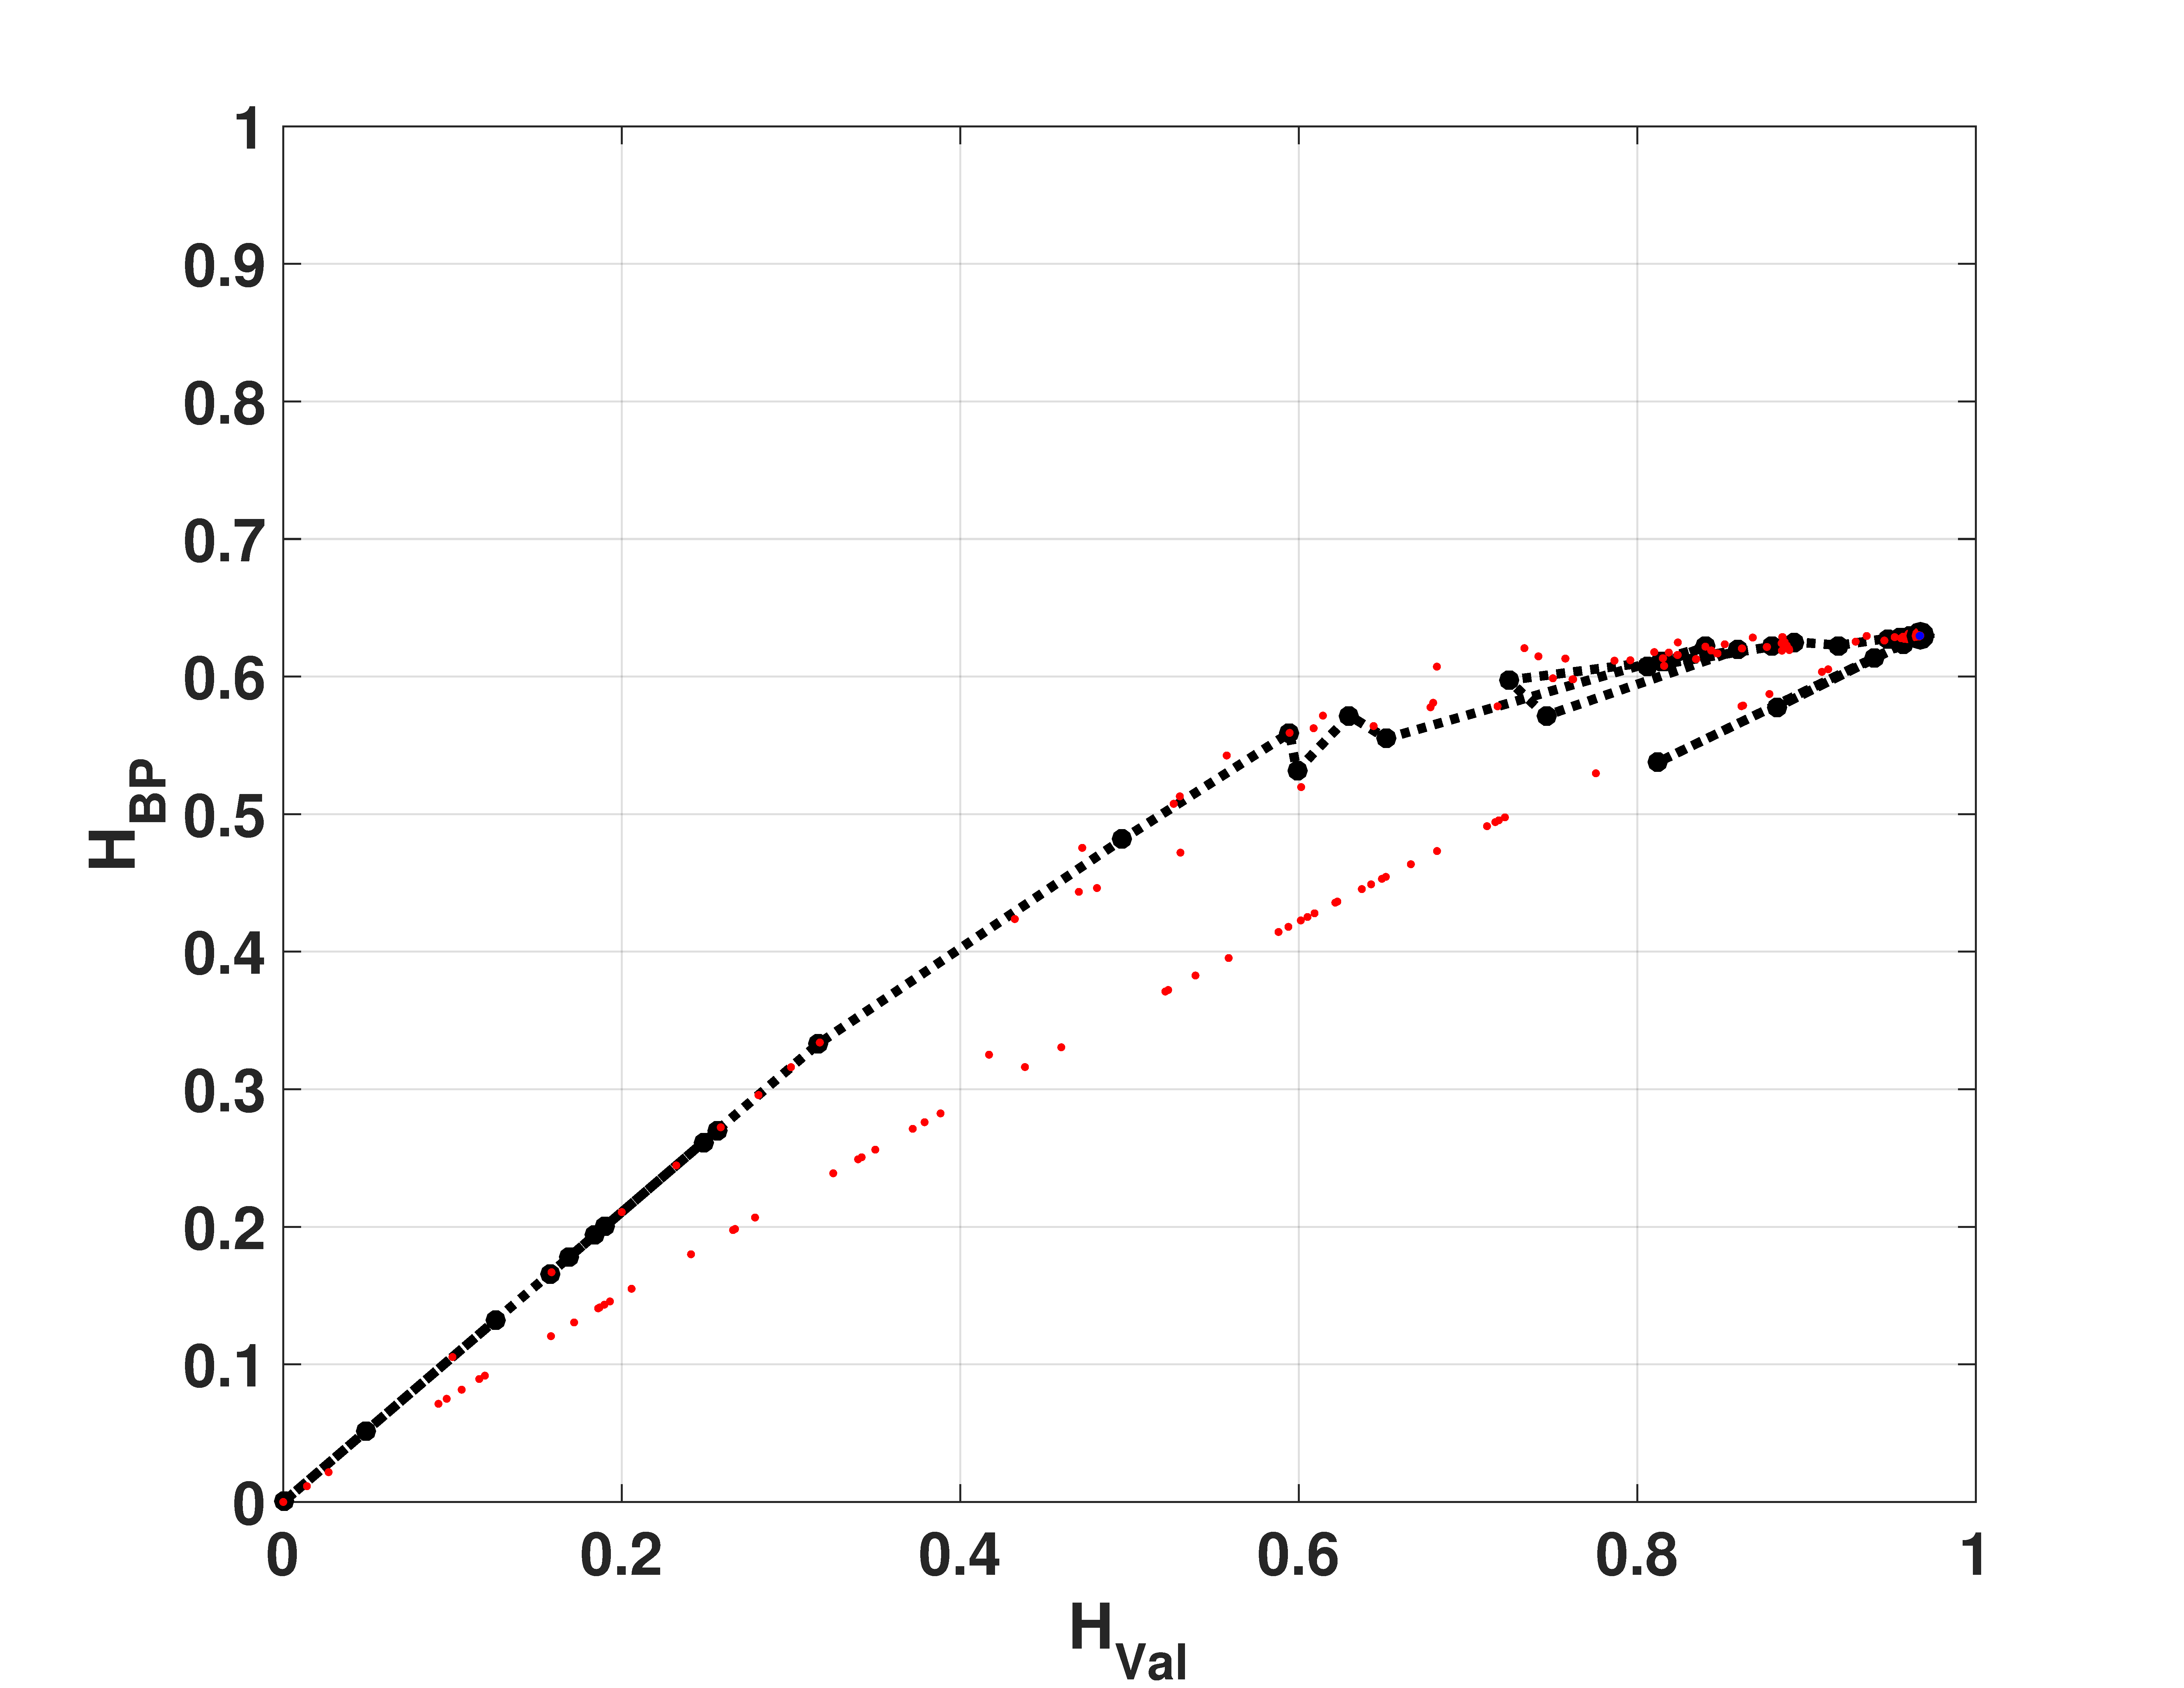
\includegraphics[width=.32\textwidth]{HbpHval_Logistico}
	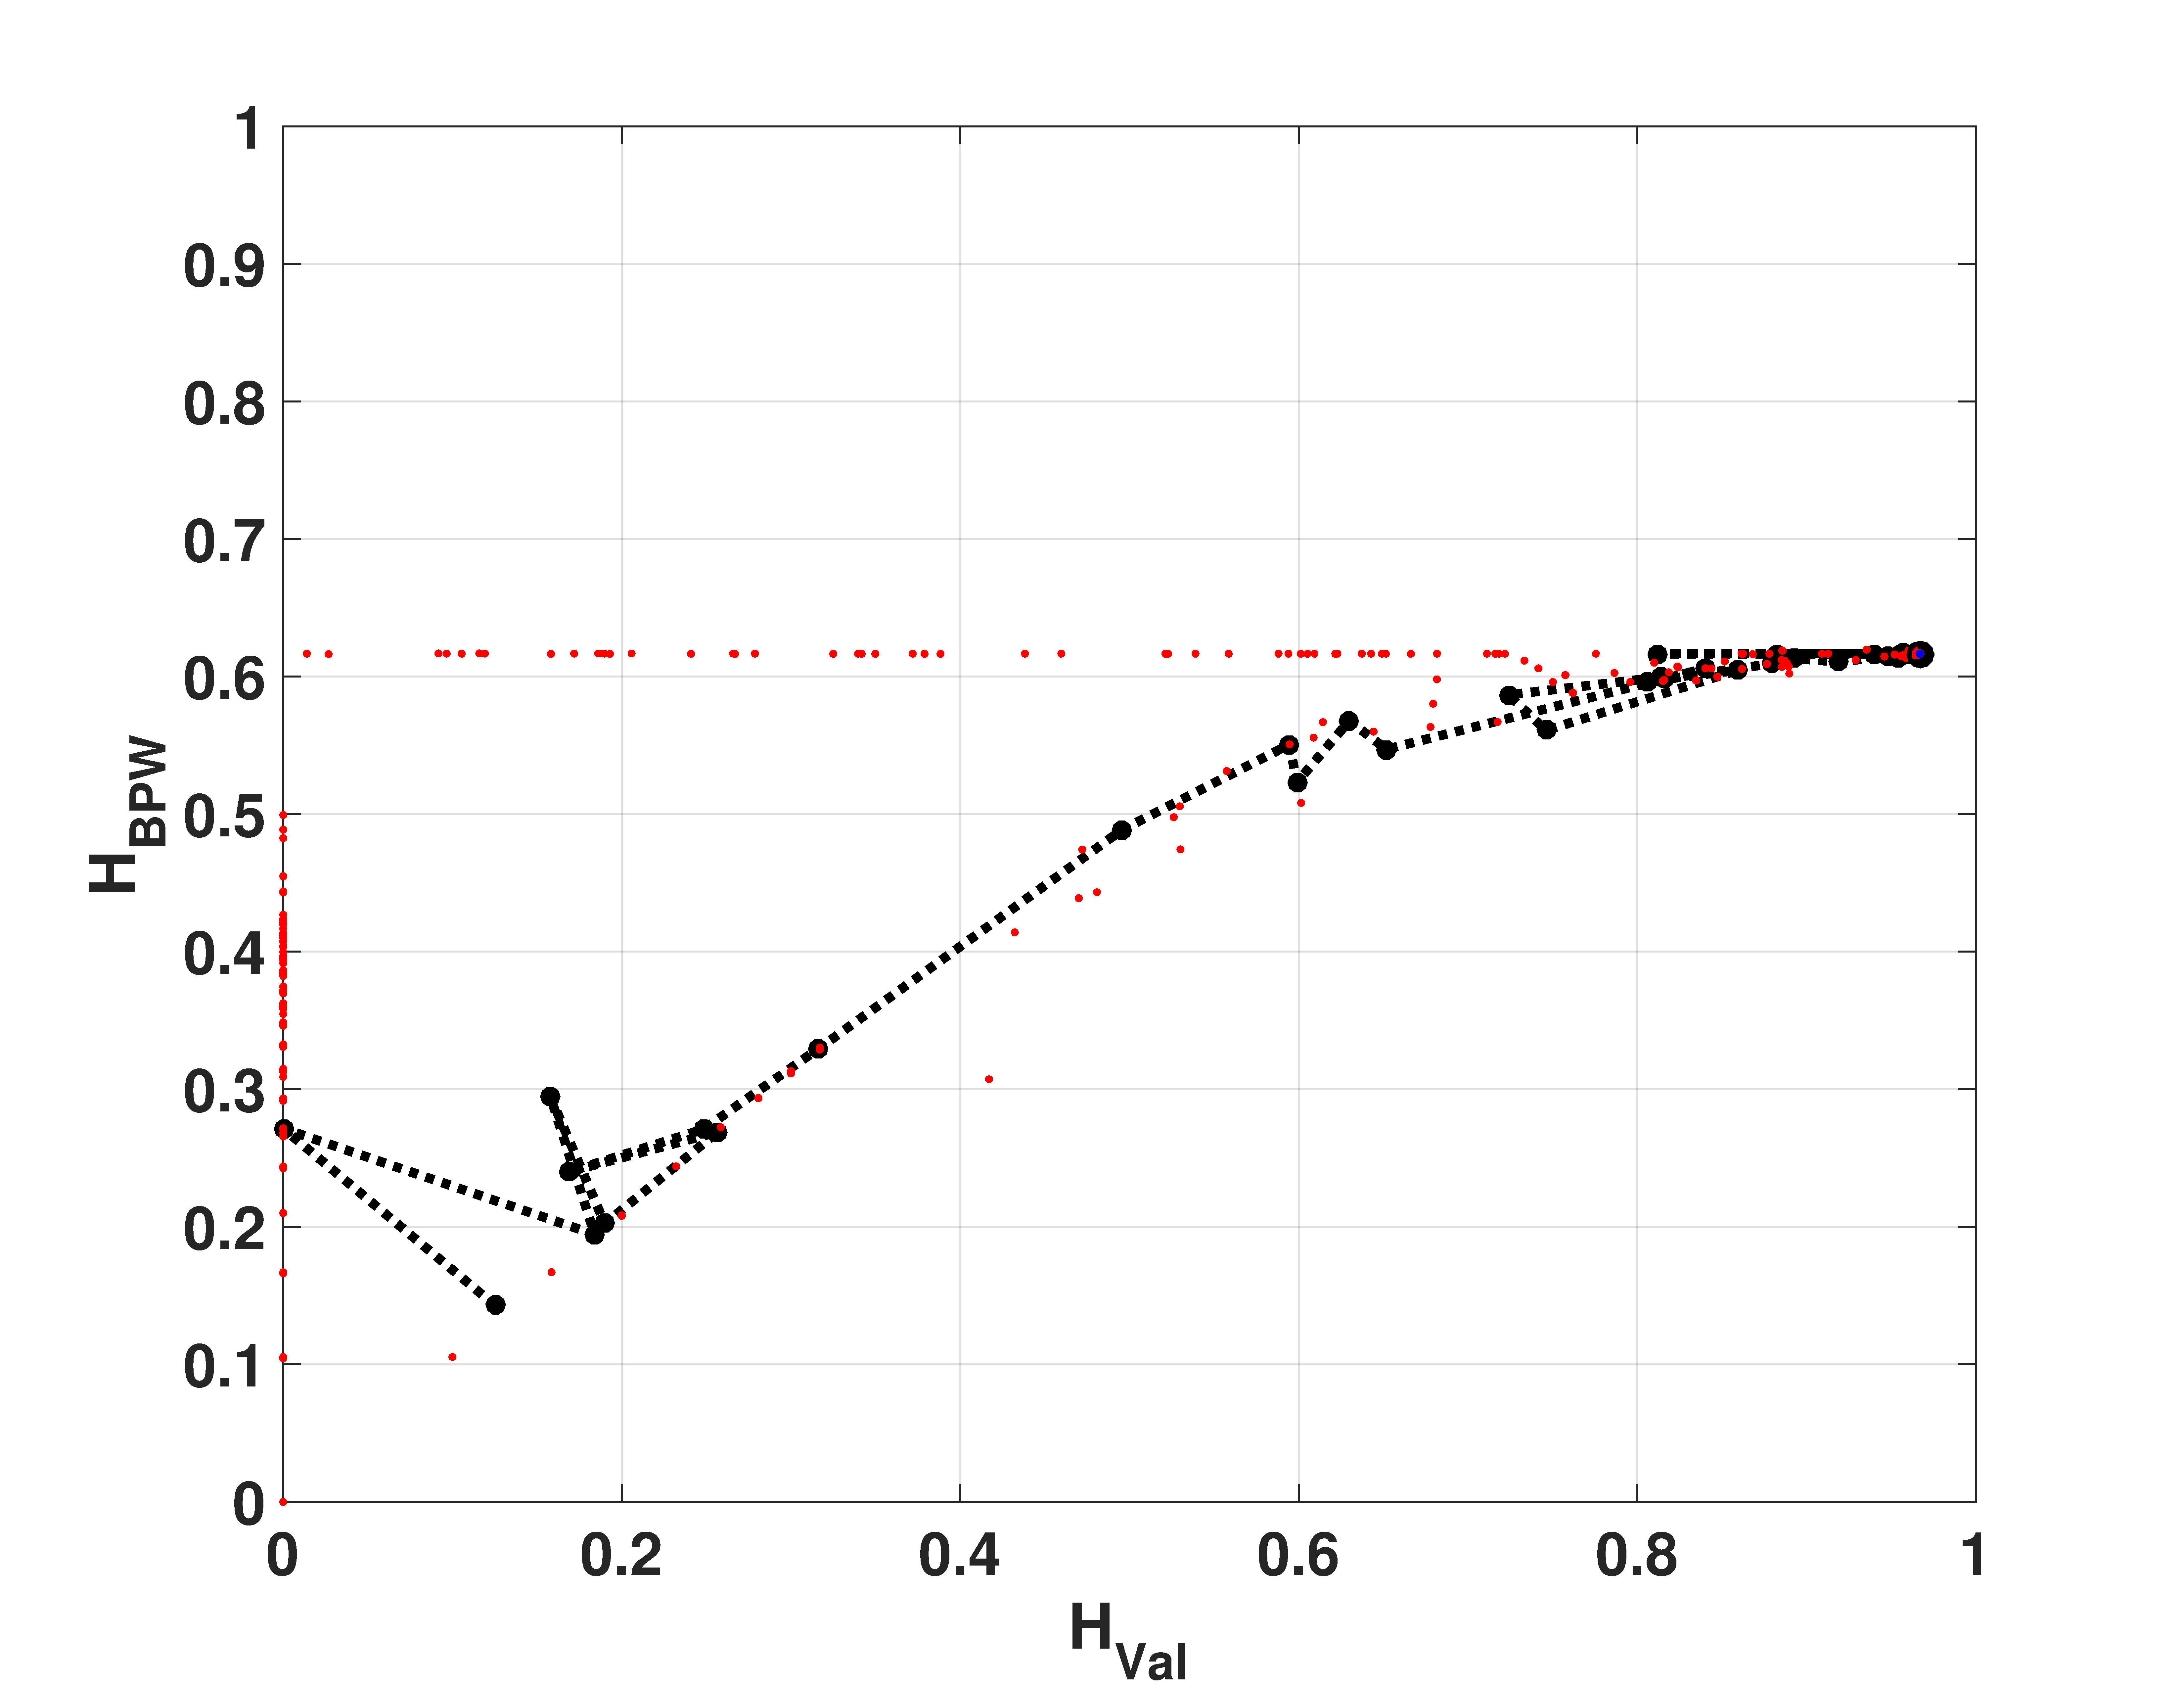
\includegraphics[width=.32\textwidth]{HbpwHval_Logistico}
	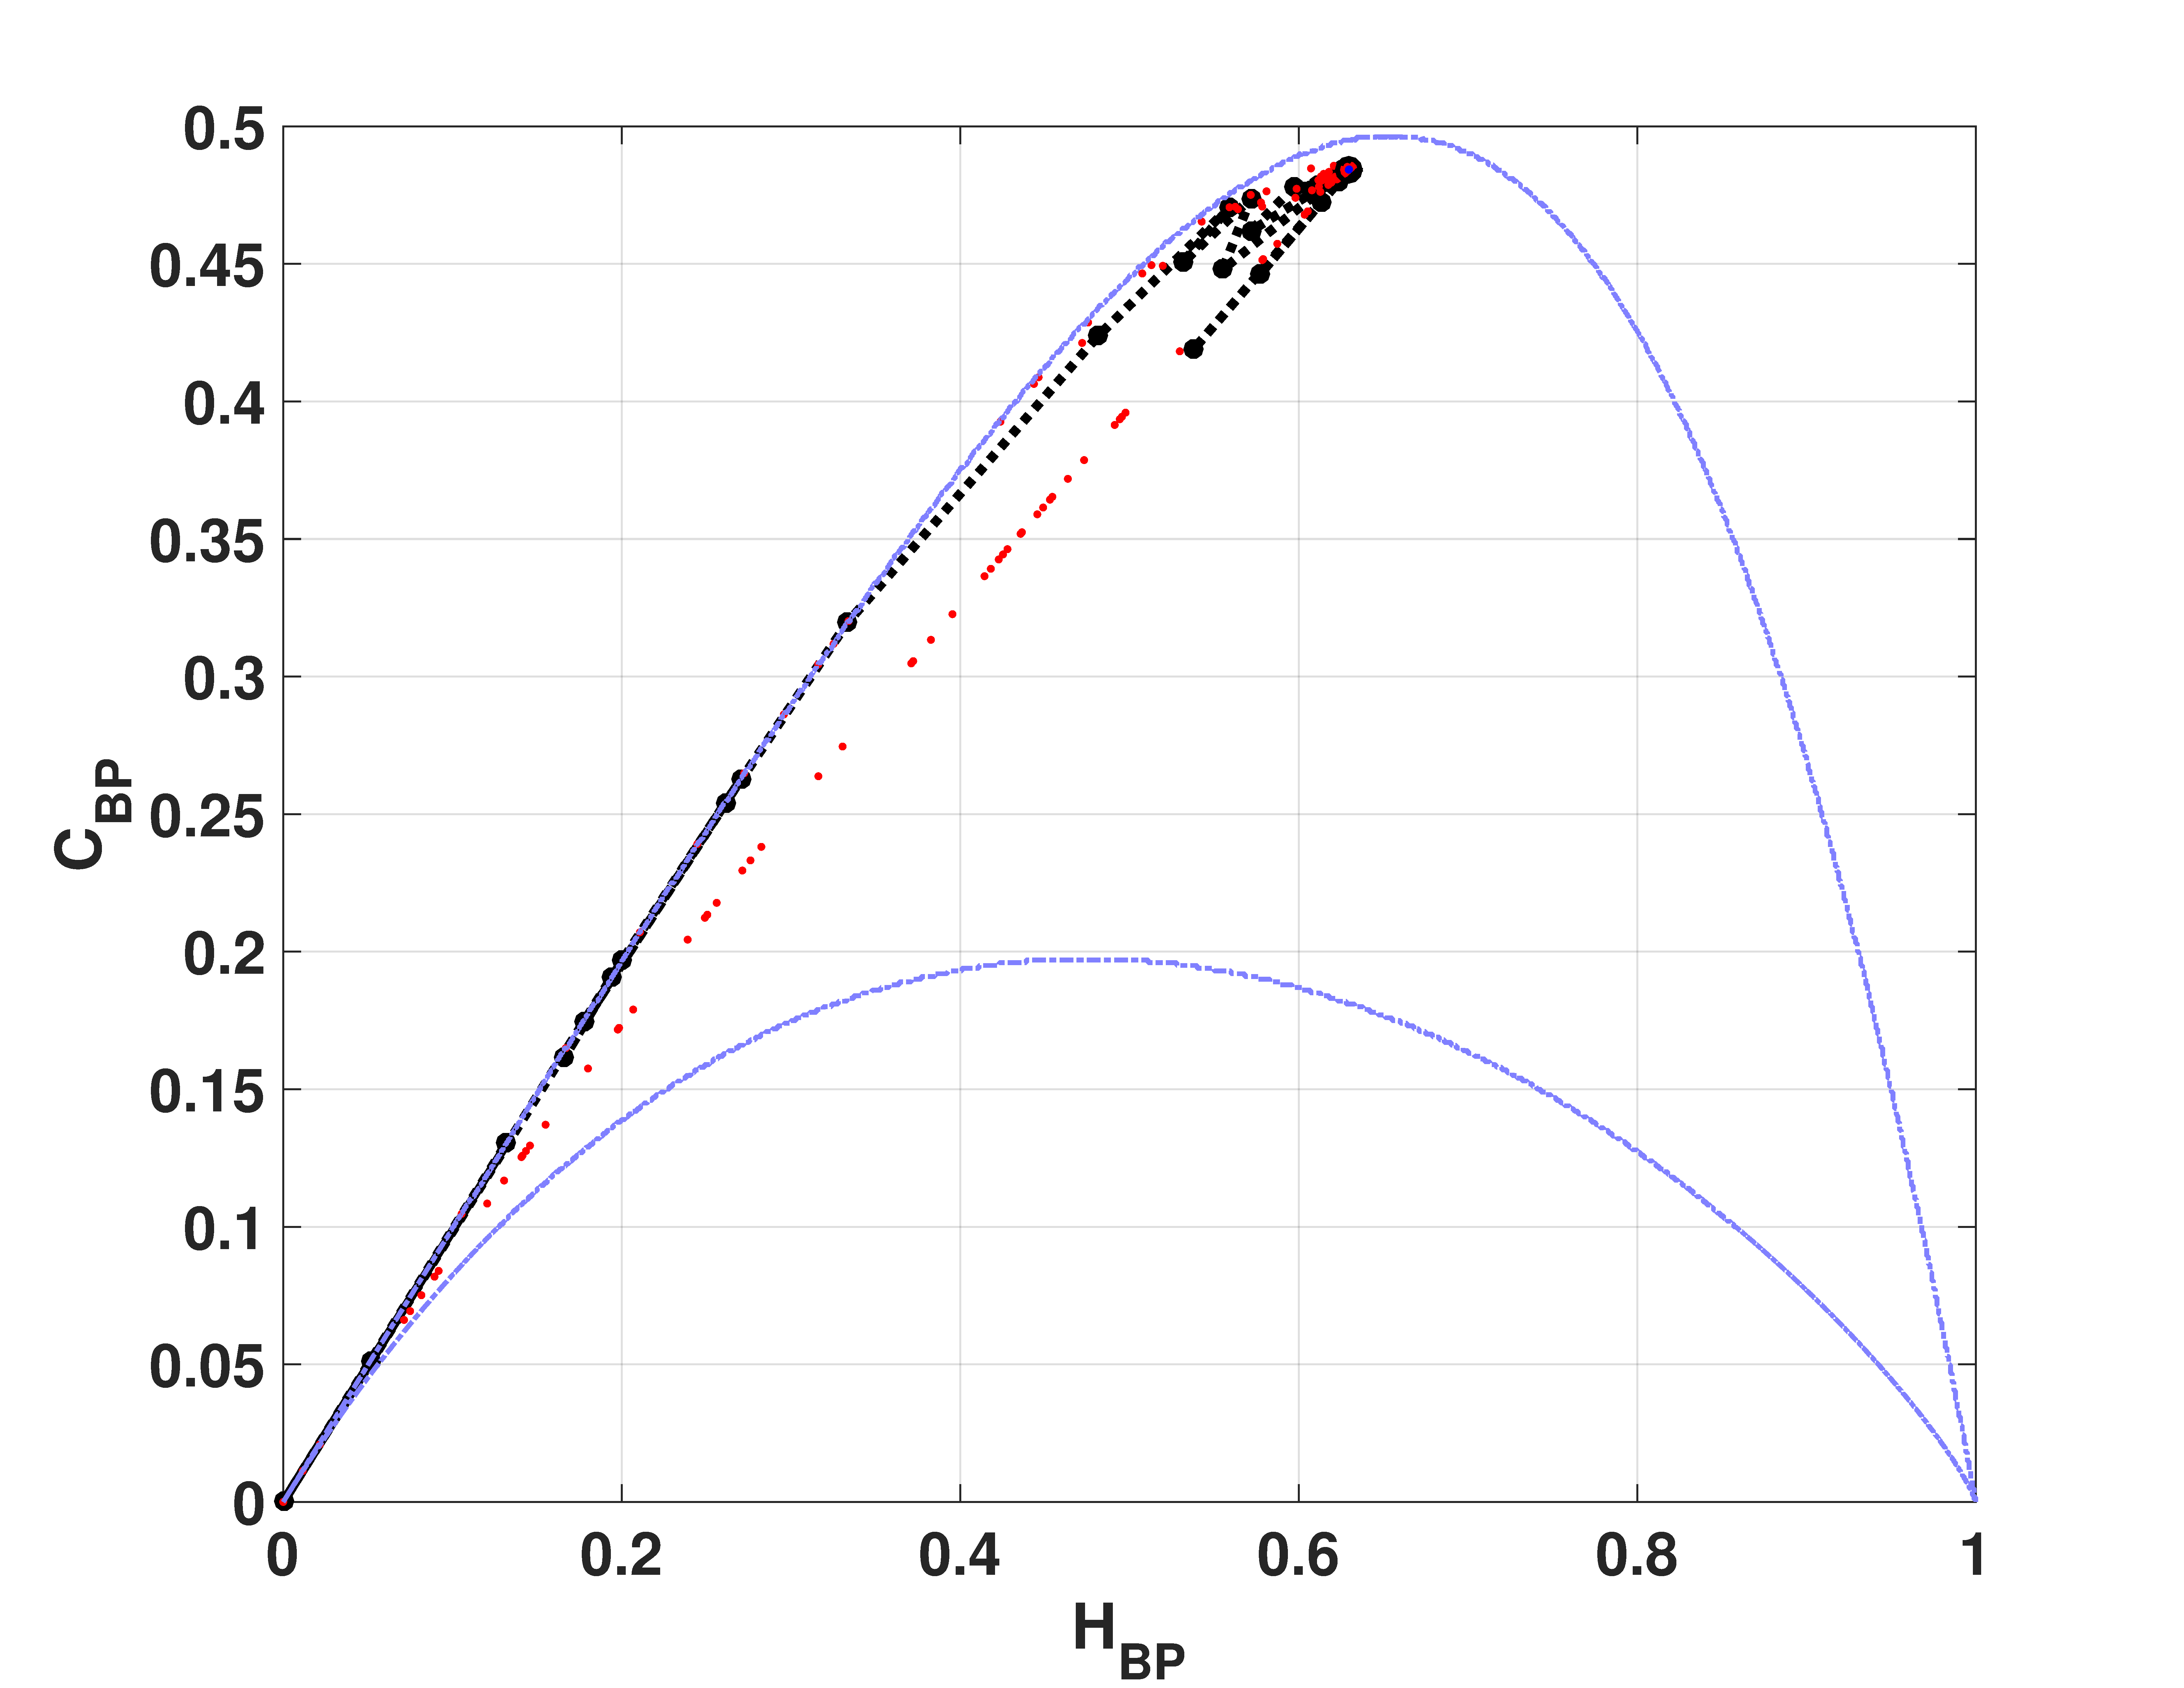
\includegraphics[width=.32\textwidth]{CbpHbp_Logistico}
	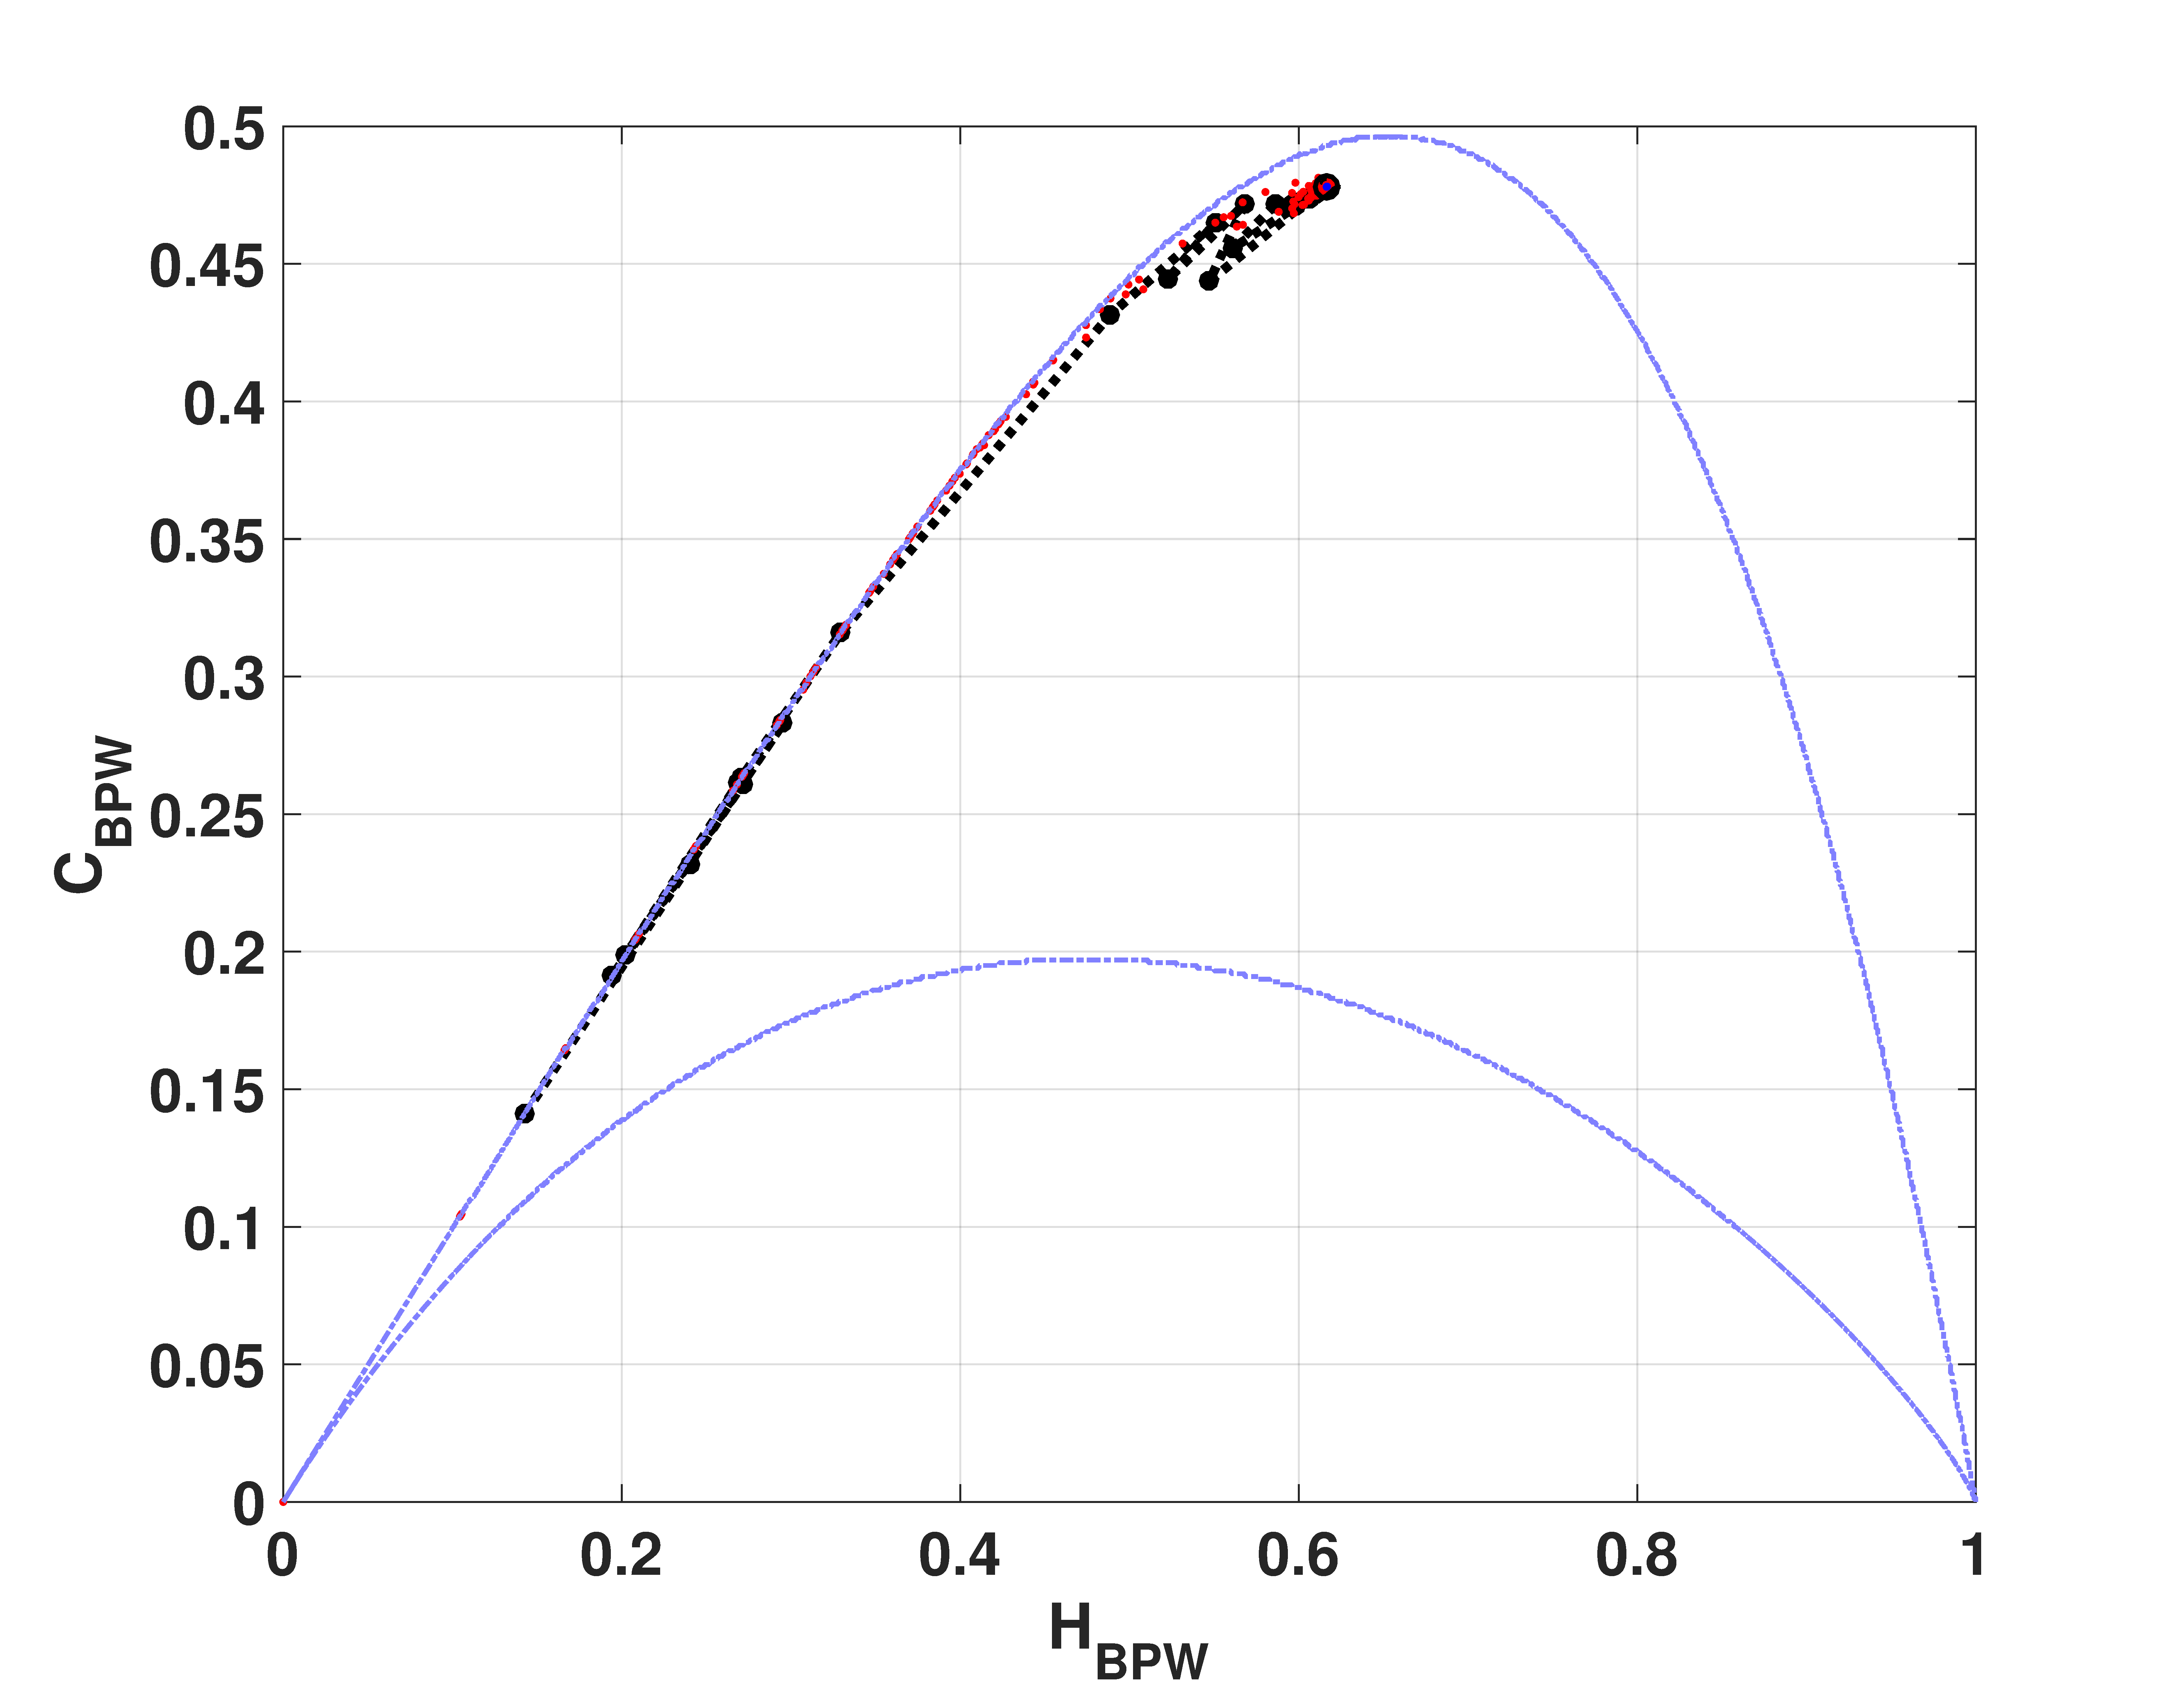
\includegraphics[width=.32\textwidth]{CbpwHbpw_Logistico}
	\caption{Statistical properties of the LOG map using binary representation: (a) $H_{hist}$ vs $P$ (b) $H_{BP}$ vs $P$ (c) $C_{BP}$ vs $P$ (d) Number of missing ordering patterns $MP$ vs $P$. In Figures (a) to (d) dashed line correspond to floating point numbers. (d) representation in the $H_{hist},H_{BP}$ plane in the the decimal numerical system.  The star represents the state for floating points numbers. (e) representation in the $H_{hist},H_{BP}$ plane. The star represents the state for floating point numbers; (f) representation in the $H_{BP},C_{BP}$ plane.  The star represents the state for floating points numbers. (f) representation in the $H_{BP},C_{BP}$ plane for binary numerical system.  The star represents the state for floating points numbers. } \label{fig:LOGbinario}
\end{figure}
